\section{统计推断部分}
\begin{center}
    Instructor: Jiangdian Wang
\end{center}

    \textbf{Statistical Inference}: Given sample $ X=(x_{1},x_{2},\ldots,x_{n})  $, we want to estimate some features of the population. This part focus on parametric statistical inference, thus our task is to estimate/testing parameters.

\begin{point}
    Example of statistical inference
\end{point}

\begin{itemize}[topsep=2pt,itemsep=0pt]
    \item Sample item $ x_i $, estimate its mean and variance
    \item Sample item $ x_i=(\vec{x_i},y_i) $, use multivariate linear model $ Y\sim \vec{X}'\beta +\beta _0 $, estimate slope \& intercept $ \beta  $ and variance $ \sigma ^2 $
\end{itemize}

        
\begin{point}
    Two main tasks of Statistical Inference
\end{point}

    \begin{itemize}[topsep= 2 pt,itemsep= 0 pt,parsep= 0 pt]
        \item Parameter Estimation
        \begin{itemize}
            \item Point Estimation: {\autoref{SectionPointEstimation}}
            \item Interval Estimation: {\autoref{SectionIntervalEstimation}}
        \end{itemize}
        \item Hypothesis Testing: {\autoref{SectionHypothesisTesting}}
    \end{itemize}

\subsection{Statistical Model and Statistics}\label{SectionStatisticalModelandStatistics}
    Random sample comes from population $X$. In parametric model case, we have population distribution family:
    \begin{equation}\mathscr{F}=\{f(x;\vec{\theta})|\vec{\theta}\in\Theta\}\end{equation}

    where \text{parameter} $\vec{\theta}$ reflect some quantities of population (e.g. mean, variance, etc.), each $\vec{\theta}$ corresponds to a distribution of population $X$.
    
    Sample space\index{Sample Space}: Def. as $\mathscr{X}=\{\{x_1,x_2,\ldots,x_n\},\forall x_i\}$, then $\{X_i\}\in\mathscr{X}$ is random sample from population $X\sim f(x;\vec{\theta})$.

    
\subsubsection{Statistics}\label{SubSectionStatistics}
    Statistic(s): function of random sample $\vec{T}(X_1,X_2,\ldots,X_n)$, \textbf{but not a function of parameter}.\index{Statistics}
    
    Some useful statistics, e.g.
    \begin{itemize}
        \item Sample mean (Consider $X_i$ i.i.d.)
        \begin{equation}
            \bar{X}=\frac{1}{n}\sum_{i=1}^n X_i
        \end{equation}
        \item Sample variance
        \begin{equation}
            S^2=\frac{1}{n-1}\sum_{i=1}^n(X_i-\bar{X})^2  
        \end{equation}
        \item Sample moments
        \begin{itemize}
            \item Origin moment
            \begin{equation}
                a_{n,k}=\frac{1}{n}\sum_{i=1}^k X_i^k\qquad k=1,2,3,\ldots    
            \end{equation}
            \item Center moment
            \begin{equation}
                m_{n,k}=\frac{1}{n}\sum_{i=1}^n (X_i-\bar{X})^k\qquad k=2,3,4,\ldots    
            \end{equation}
        \end{itemize}
        \item Order statistics\index{Order Statistics}
        \begin{equation}
            (X_{(1)},X_{(2)},\ldots,X_{(n)}),\,\text{for }X_{(1)}\leq X_{(2)} \leq \ldots\leq X_{(n)}    
        \end{equation}
        \item Sample $p$-fractile
        \begin{equation}
            m_p=X_{(m)},\quad m=\left\lfloor (n+1)p\right\rfloor    
        \end{equation}
        \item Sample coefficient of variation
        \begin{equation}
            \hat{\nu}=\frac{S}{\bar{X}}    
        \end{equation}
        \item Skewness and Kurtosis
        \begin{equation}
            \hat{g}_1=\frac{m_{n,3}}{m_{n,2}^{3/2}}\qquad \hat{g}_2=\frac{m_{n,4}}{m_{n,2}^2}    -3
        \end{equation}
    \end{itemize}

    \begin{point}
        Properties
    \end{point}
    
        

    Statistic $T$ is a function of random sample $\{X_i\}$, thus has distribution (say $g_T(t)$) called \textbf{Sampling Distribution}.\index{Statistics!Sampling Distribution}

        For $X_i$ i.i.d. from $X\sim f(x)$ with population mean $\mu$ and variance $\sigma^2$
    \begin{itemize}
        \item Calculation of sample variance $S^2$
        \begin{equation}(n-1)S^2=\sum_{i=1}^n x_i^2-n\bar{x}^2\end{equation}
        \item $\mathbb{E}$ and $var$ of $\bar{X}$ and $S^2$
        \begin{equation}\mathbb{E}(\bar{X})=\mu\qquad var(\bar{X})=\frac{\sigma^2}{n}\qquad \mathbb{E}(S^2)=\sigma^2\end{equation}
    \end{itemize}

    Further if $X_i$ i.i.d. from $X\sim N(\mu,\sigma^2)$ where $\mu$ and $\sigma^2$ unknown.
    \begin{itemize}
        \item Independence of $\bar{X}$ and $S^2$ 
            \begin{equation}
            \bar{X}\independent S^2
            \end{equation}
        \begin{itemize}[topsep=6pt,itemsep=4pt]
        \item Distribution of $\bar{X}={\displaystyle\frac{1}{n}\sum_{i=1}^n X_i}$
        \begin{equation}\bar{X}\sim N(\mu,\frac{\sigma^2}{n})\end{equation}
        \item Distribution of $S^2={\displaystyle\frac{1}{n-1}\sum_{i=1}^n(X_i-\bar{X})^2}$
        \begin{equation}\frac{(n-1)S^2}{\sigma^2}\sim\chi^2_{n-1}\end{equation}
        \end{itemize}     
        Comment: the independence here can explain the $ n-1 $ degree of freedom of $ \chi^2_{n-1} $   
    \end{itemize}

\subsubsection{Exponential Family}\label{SubSectionExponentialFamily}
        Def. $\mathscr{F}_\Theta=\{f(x;\vec{\theta}|\vec{\theta}\in\Theta)\}$ is \textbf{Exponential Family} if $f(x;\vec{\theta})$ has the form as\index{EF (Exponential Family)}
\begin{equation}
    f(x;\vec{\theta})=C(\vec{\theta})h(x)\exp \left[  \sum_{i=1}^k Q_i(\vec{\theta})T_i(x) \right]\quad\vec{\theta}\in\Theta
\end{equation}    

    Or equivalently express $ c(\vec{\theta })=\ln C(\vec{\theta }) $:
\begin{equation}
    f(x;\vec{\theta})=h(x)\exp \left[  \sum_{i=1}^k Q_i(\vec{\theta})T_i(x) +c(\vec{\theta }) \right]\quad\vec{\theta}\in\Theta
\end{equation}   

    Canonical Form: Take $Q_i(\vec{\theta})=\varphi_i$, then $\vec{\varphi}=(\varphi_1,\varphi_2,\ldots,\varphi_k)=$$(Q_1(\vec{\theta}),Q_2(\vec{\theta}),\ldots,Q_k(\vec{\theta}))$ is a transform from $\Theta$ to $\Theta^*$, s.t. $\mathscr{F}$ has canonical form, i.e.
    \begin{equation}\label{EqaExponentialDistributionFamily}
        f(x;\vec{\varphi})=C^*(\vec{\varphi})h(x)   \exp\left[  \sum_{i=1}^k \varphi_i T_i(x) \right] \quad \vec{\varphi}\in\Theta^*
    \end{equation}

    $\Theta^*$ is canonical parameter space.

    

\begin{point}
    Why we need exponential family? It has some nice properties.
\end{point}




\subsubsection{Sufficient and Complete Statistics}\label{SubSectionSufficient_CompleteStatistics}
    Note: For simplification, the following parts denote $\vec{\theta},\vec{T},\ldots$  as $\theta,T,\ldots$ etc.
    \begin{itemize}
        \item[$\blacktriangleright$] \index{Statistics!Sufficient Statistic}A \textbf{Sufficient Statistic} $T(\vec{X})$ for $\theta$ contains all the information of sample when infer $\theta$, i.e.
        \begin{equation}
            f(\vec{X};T(\vec{X}))=f(\vec{X};T(\vec{X}),\theta)
        \end{equation}

        Properties
        \begin{itemize}
            \item \textbf{Factorization Thm.}\index{Factorization Thm.} $T(\vec{X})$ is sufficient \textbf{if and only if} $f_{\vec{X}}(\vec{x};\theta)=f(\vec{x};\theta)$ can be written as 
            \begin{equation}
                f(\vec{x};\theta)=g[t(\vec{x});\theta]h(\vec{x})
            \end{equation}            
            \item If $T(\vec{X})$ sufficient, then $T'(\vec{X})=g[T(\vec{X})]$ also.(require $g$ single-valued and invertible)
            \item If $T(\vec{X})$ sufficient, then $(T,T_1)$ also.
            \item Minimal sufficient statistic $T_\theta(\vec{X})$ satisfies 
            \begin{equation}
                \forall\,\text{sufficient statistic }S,\,\exists\, q_S(\cdot),\, \text{s.t.} T_\theta=q_S(S)
            \end{equation}

            A minimal sufficient statistic not always exists.

            Sufficient \& Complete $\Rightarrow $ Minimal sufficient.
            \item Usually dimension of $\vec{T}_\theta$ and $\theta$ equals.
        \end{itemize}
        
        Sufficient statistic is \textbf{not} unique.



        \item[$\blacktriangleright$] A \textbf{Complete Statistic}\index{Statistics!Complete Statistic} $T(\vec{X})$ for $\theta$ satisfies
        \begin{equation}
            \forall\theta\in\Theta\, ;\,\forall\varphi\text{ satisfies }\mathbb{E}[\varphi(T(\vec{X}))]=0\text{, we have }\mathbb{P}[\varphi(T)=0;\theta]=1
        \end{equation}

        Explanation: $T\sim g_T(t)$. Rewrite as
        \begin{equation}
            \int\varphi (t) g_T(t)\,\mathrm{d} t=0  \, \Rightarrow\varphi(T)=0 \text{  a.s. }\,\forall\,\theta
        \end{equation}

        i.e. \underline{$\mathrm{span}\{g_T(t);\forall\theta\}$ is a complete space}. Or to say that $\nexists$ none-zero $\varphi(t)$ so that $\mathbb{E}(\varphi(T))=0$ (unbiased estimation)

        \begin{equation}
            \varphi(T)\neq 0 \,\,\forall \theta\Rightarrow \mathbb{E}[\varphi(T(\vec{X}))]\neq 0  
        \end{equation}

        So make sure the uniqueness of unbiased estimation of $\hat{\theta}$ using $T$.

        Properties
        \begin{itemize}
            \item If $T(\vec{X})$ complete, then $T^\prime(\vec{X})=g[T(\vec{X})]$ also.(require $g$ measurable)

            \item A complete statistic not always exists.
        \end{itemize}
        \item[$\blacktriangleright$]\index{Statistics!Ancillary Statistic}  An \textbf{Ancillary Statistic} $S(\vec{X})$ is a statistic whose distribution does not depend on $\theta$
        
        \textbf{Basu Thm.}\index{Basu Thm.}: $\vec{X}=(X_1,X_2,\ldots,X_n)$ is sample from $\mathscr{F}=\{f(x;\theta),\theta\in\Theta\}$. $T(\vec{X})$ is a complete and minimal sufficient statistic, $S(\vec{X})$ is ancillary statistic, then $S(\vec{X})\independent T(\vec{X})$.

        \item[$\blacktriangleright$] Exponential family: For $\vec{X}=(X_1,X_2,\ldots,X_n)$ from exponential family with canonical form, i.e.
    \begin{equation}
        f(\vec{x};\theta)=C(\theta)h(\vec{x})\exp\left[\sum_{i=1}^k \theta_i T_i(\vec{x})\right] ,\quad \theta\in\Theta
    \end{equation}

    Then if $\Theta\in\mathbb{R}^k$ interior point exists, then $T(\vec{X})=(T_1(\vec{X}),T_2(\vec{X}),\ldots,T_k(\vec{X}))$ is sufficient \& complete statistic.


\end{itemize} 




\subsection{Point Estimation}\label{SectionPointEstimation}
    For parametric distribution family $\mathscr{F}=\{f(x,\theta),\theta\in\Theta\}$, random sample $\vec{X}=(X_1,X_2,\ldots,X_n)$ from $\mathscr{F}$. $g(\theta)$ is a function defined on $\Theta$. 

    Mission: use sample $\{X_i\}$ to estimate $g(\theta)$, called \textbf{Parameter Estimation}.

    \begin{equation}
        \text{Parameter Estimation}\begin{cases}
            \text{Point Estimation}& \surd\\
            \text{Interval Estimation}&
        \end{cases}    
    \end{equation}

    Point estimation: when estimating $\theta$ or $g(\theta)$, denote the estimator (defined on sample space $\mathscr{X}$) as
    \begin{equation}
        \hat{\theta}(\vec{X})\qquad \hat{g}(\vec{X})    
    \end{equation}

    Estimator is a statistic, with sampling distribution.
\subsubsection{Optimal Criterion}\label{SubSectionOptimalCriterion}
        Some nice properties of estimators (that we expect)
    \begin{itemize}
        \item Unbiasedness
        \begin{equation}
            \mathbb{E}(\hat{\theta})=\theta   \quad \text{or}\quad \mathbb{E}(\hat{g}(\vec{X})) =g(\theta)
        \end{equation}

        Otherwise, say $\hat{\theta}$ or $\hat{g}$ biased. Def. \textbf{Bias}: $\mathbb{E}(\hat{\theta})-\theta$

        Asymptotically unbiasedness with $ n $ as sample size
        \begin{equation}
            \lim_{n\to\infty}  E(\hat{g}_n(\vec{X})) =g(\theta)  
        \end{equation}
        \item Efficiency: say $\hat{g}_1(\vec{X})$ is more efficient than $\hat{g}_2(\vec{X})$, if
        \begin{equation}
            var(\hat{g}_1)\leq var(\hat{g}_2)  \quad\forall\theta\in\Theta  
        \end{equation}
        \item Mean Squared Error (MSE)\index{MSE (Mean Squared Error)}: Bias-Variance Trade-Off
        \begin{equation}\label{EqaMSEExpansion}
            \text{MSE}=\mathbb{E}[(\hat{\theta}-\theta)^2]=var(\hat{\theta})+[Bias(\hat{\theta})]^2
        \end{equation}

        For unbiased estimator, i.e. $Bias(\hat{\theta})=0$, we have
        \begin{equation}
            \text{MSE}=\mathbb{E}[(\hat{\theta}-\theta)^2]=var(\hat{\theta})
        \end{equation}
        \item (Weak) Consistency
        \begin{equation}
            \lim_{n\to\infty}\mathbb{P}(|\hat{g}_n(\vec{X})-g(\theta)|\geq \varepsilon)=0\quad\forall\varepsilon>0    
        \end{equation}
        \item Asymptotic Normality
    \end{itemize}


\subsubsection{Method of Moments}\label{SubSectionMoM}
    Review: Population moments \& Sample moments\index{MoM (Method of Moments)}
    \begin{align*}
        \alpha_k&=\mathbb{E}(X^k)&\mu_k&=\mathbb{E}[(X-\mathbb{E}(X))^k]\\
        a_{n,k}&=\hat{\alpha }_k =\frac{1}{n}\sum_{i=1}^nX_i^k&m_{n,k}&=\hat{\mu }_k=\frac{1}{n}\sum_{i=1}^n(X_i-\bar{X})^k
    \end{align*}

    Property: $a_{n,k}$ is the unbiased estimator of $\alpha_k$.(while $m_{n,k}$ unually biased for $\mu_k$)

    For sample $\vec{X}=(X_1,X_2,\ldots,X_n)$ from $\mathscr{F}=\{f(x;\theta,\theta\in\Theta)\}$, unknown parameter (or its function) $g(\theta)$ can be written as
    \begin{equation}
        g(\theta)=G(\alpha_1,\alpha_2,\ldots,\alpha_k;\mu_2,\mu_3,\ldots,\mu_l)    
    \end{equation}

    Then its \textbf{Moment Estimate} $\hat{g}(\vec{X})$ is
\begin{equation}
    \hat{g}(\vec{X})=G(a_{n,1},a_{n,2},\ldots,a_{n,k};m_{n,2},m_{n,3},\ldots,m_{n,l}) 
\end{equation}

    Example: coefficient of variance \& skewness 
    \begin{equation}\hat{\nu}=\dfrac{S}{\bar{X}}\qquad\hat{\beta}_1=\dfrac{m_{n,3}}{m_{n,2^{3/2}}}=\sqrt{n}{\displaystyle\frac{\displaystyle{\sum_{i=1}^n(X_i-\bar{X})^3}}{\displaystyle{\left[\sum_{i=1}^n(X_i-\bar{X})^2\right]^{\frac{3}{2}}}  }}\end{equation}

    \begin{point}
        Note:
    \end{point}
    
        
    \begin{itemize}
        \item $G$ may not have explicit expression.
        \item Moment estimate may not be unique.
        \item If $G={\displaystyle\sum_{i=1}^kc_i\alpha_i}$ (linear combination of $\alpha$, without $\mu$), then $\hat{g}(\vec{X})={\displaystyle\sum_{i=1}^kc_ia_{n,i}}$ unbiased.
        
        \qquad Usually $\hat{g}(\vec{X})$ is asymptotically unbiased.
        \item For small sample, not so accurate.
        \item May not contain all the information about $\theta$, i.e. may not be sufficient statistic.
        \item Do not require a statistic model.
    \end{itemize}


\subsubsection{Maximum Likelihood Estimation}\label{SubSectionMLE}
    \index{MLE (Maximum Likelihood Estimation)}For sample $\vec{X}=(X_1,X_2,\ldots,X_n)$ with distribution $f(\vec{x};\theta)$ from $\mathscr{F}=\{f(x;\theta),\theta\in\Theta\}$ , def. \textbf{Likelihood Function} $L(\theta;\vec{x})$, defined on $\Theta$ (as a function of $\theta)$\index{Likelihood Function}
    \begin{equation}
        L(\theta;\vec{x})=f(\vec{x};\theta)\qquad \theta\in\Theta,\,\vec{x}\in\mathscr{X}    
    \end{equation}

    Also def. log-likelihood function $l(\theta;\vec{x})=\ln L(\theta;\vec{x})$.

    If estimator $\hat{\theta}=\hat{\theta}(\vec{X})$ satisfies
    \begin{equation}
        L(\hat{\theta};\vec{x})=\sup_{\theta\in\Theta}L(\theta;\vec{x}),\quad \vec{x}\in\mathscr{X}
    \end{equation}

    Or equivalently take $l(\theta;\vec{x})$ instead of $L(\theta;\vec{x})$.

    Then $\hat{\theta}=\hat{\theta}(\vec{X})$ is a \textbf{Maximum Likelihood Estimate}(MLE) of $\theta=(\theta_1,\theta_2,\ldots,\theta_k)$

    How to identify MLE?
    \begin{itemize}
        \item Differentiation: Fermat Lemma
        \begin{equation}
            \frac{\partial L}{\partial \theta_i}\bigg|_{\theta=\hat{\theta}}=0\qquad \frac{\partial^2 L}{\partial \theta_i \partial \theta_j}\bigg|_{\theta=\hat{\theta}}\text{negative definite}\qquad \forall i,j=1,2,\ldots,k
        \end{equation}
        \item Graphing method.
        \item Numerically compute maximum.
    \end{itemize}

    \begin{point}
        Some properties of MLE
    \end{point}
    
        
    \begin{itemize}
        \item (Depend on the case, not always) unbiased.
        \item Invariance of MLE\index{Invariance of MLE}: If $\hat{\theta}$ is MLE of $\theta$, invertible function $g(\theta)$, then $g(\hat{\theta})$ is MLE of $g(\theta)$.
        \item MLE and Sufficiency: $T=T(X_1,X_2,\ldots,X_n)$ is a sufficient statistic of $\theta$, if MLE of $\theta$ exists, say $\hat{\theta}$, then $\hat{\theta}$ is a function of $T$, i.e.
        \begin{equation}  
            \hat{\theta}=\hat{\theta}(\vec{X})=\hat{\theta}^*(T(\vec{X}))    
        \end{equation}
        \item Asymptotic Normality: 
        \begin{equation}
            \sqrt{n}(\hat{\theta}_n-\theta) \xrightarrow[]{d}N(0,\sigma^2_\theta),\quad \sigma^2_\theta=\frac{1}{\mathbb{E}_\theta[\frac{\partial}{\partial\theta}\ln f(\vec{X};\theta)]^2}   
        \end{equation}

        i.e.
        \begin{equation}
            \hat{\theta}_n\xrightarrow[]{d}N(\theta,\frac{\sigma^2_\theta}{n})    
        \end{equation}
        
    \end{itemize}

    \begin{point}
        Comparison: MoM and MLE
    \end{point}
    
        
    \begin{itemize}
        \item MoM do not require statistic model; MLE need to know PDF.
        \item MoM is more robust than MLE.
    \end{itemize}


    MLE in Exponential Family:

        For sample $\vec{X}=(X_1,X_2,\ldots,X_n)$ from canonical exponential family $\mathscr{F}=\{f(x;\theta),\theta\in\Theta\}$
        \begin{equation}
            f(x;\theta)=C(\theta)h(x)\exp\left[\sum_{i=1}^k\theta_iT_i(x)\right]\quad \theta=(\theta_1,\ldots,\theta_k)\in\Theta
        \end{equation}

        Likelihood function $L(\theta,\vec{x})=\prod_{j=i}^nf(x_j;\theta)$ and log-likelihood function $l(\theta,\vec{x})$
        \begin{align*}
            L(\theta,\vec{x})&=C^n(\theta)\prod_{j=1}^nh(x_j)\exp\left[\sum_{i=1}^k\theta_i\sum_{j=1}^n T_i(x_j)\right]\\
            \ell(\theta,\vec{x})&=n\ln C(\theta)+\sum_{j=1}^n\ln h(x_j)+\sum_{i=1}^k\theta_i\sum_{j=1}^nT_i(x_j)
        \end{align*}

        Solution of MLE: (Require $\hat{\theta}\in\Theta$)
        \begin{equation}
            \frac{n}{C(\theta)}\frac{\partial C(\theta)}{\partial \theta_i}\bigg|_{\theta=\hat{\theta}}=-\sum_{j=1}^nT_i(x_j),\quad i=1,2,\ldots,k    
        \end{equation}


\subsubsection{Uniformly Minimum Variance Unbiased Estimator}\label{SubSectionUMVUE}
        \index{UMVUE (Uniformly Minimum Variance Unbiased Estimator)}MSE: For $\hat{g}(\vec{X})$ is estimate of $g(\theta)$ ,then MSE
        \begin{equation}
            \mathrm{MSE}(\hat{g}(\vec{X}))=\mathbb{E}[(\hat{g}(\vec{X})-g(\theta))^2]=var(\hat{g})+[Bias(\hat{g})]^2
        \end{equation}

        Note:
    Unbiased estimator (i.e. $Bias(\hat{g})=0$) is not unique; ang not always exists.


    


        Now only consider unbiased estimators of $g(\theta)$ exists, say $\hat{g}(\vec{X})$, then
        \begin{equation} \mathrm{MSE}(\hat{g}(\vec{X}))=var(\hat{g}(\vec{X})) \end{equation}

        If $\forall$ unbiased estimate $\hat{g}\prime(\vec{X})$, $\hat{g}$ satisfies
        \begin{equation}
            var[\hat{g}(\vec{X})]\leq var[\hat{g}\prime(\vec{X})]    
        \end{equation}

\begin{point}
        Then $\hat{g}(\vec{X})$ is \textbf{Uniformly Minimum Variance Unbiased Estimator(UMVUE)} of $g(\theta)$
\end{point}


        How to determine UMVUE? (Not an easy task)
        \begin{itemize}
            \item Zero Unbiased Estimate Method
            \item Sufficient and Complete Statistic Method
            \item Cramer-Rao Inequality
        \end{itemize}

\begin{enumerate}
\item \textbf{Zero Unbiased Estimate Method}
            
    Let $\hat{g}(\vec{X})$ be an unbiased estimate with $var(\hat{g})<\infty$. If $\forall$ $\mathbb{E}(\hat{l}(\vec{X}))=0$ , $\hat{g}$ holds that
    \begin{equation}
        cov(\hat{g},\hat{l})=\mathbb{E}(\hat{g}\cdot\hat{l})=0,\quad\forall\theta\in\Theta    
    \end{equation}

    Then $\hat{g}$ is a UMVUE of $g(\theta)$ (sufficient \& necessary).





\item \textbf{Sufficient and Complete Statistic Method}

    For $T(\vec{X})$ sufficient statistic, $\hat{g}(\vec{X})$ unbiased estimate of $g(\theta)$, then 
\begin{equation}
    h(T)=\mathbb{E}(\hat{g}(\vec{X})| T)    
\end{equation}

    is an unbiased estimate of $g(\theta)$ and $var(h(T))\leq var(\hat{g})$.

    Remark:
    \begin{itemize}
        \item A method to improve estimator.
        \item A UMVUE has to be a function of sufficient statistic.
    \end{itemize}

    \textbf{Lehmann-Scheffé Thm.}\index{LS Thm. (Lehmann-Scheffé Thm.)}: For $\vec{X}=(X_1,X_2,\ldots,X_n)$ from population $X\sim\mathscr{F}=\{f(x;\theta):\vec{\theta}\in\Theta\}$. $T(\vec{X})$ sufficient and complete, and $\hat{g}(T(\vec{X}))$ be an unbiased estimator, then $\hat{g}(T(\vec{X}))$ is the unique UMVUE.

    Can be used to construct UMVUE: given $T(\vec{X})$ sufficient and complete and some unbiased estimator $\hat{g}\prime(\theta)$ then 
    \begin{equation}
        \hat{g}(T)=\mathbb{E}(\hat{g}\prime|T)    
    \end{equation}

    is the unique UMVUE.



\item \textbf{Cramer-Rao Inequality}\index{CR Inequality (Cramer-Rao Inequality)}

    Core idea: determine a lower bound of $var(\hat{g})$.

    Consider $\theta=\theta$ (One dimension parameter); For $\{X_i\}$ i.i.d. $f(x,\theta)$: def.
    \begin{itemize}
        \item \textbf{Score function}\index{Score Function}: Reflects the steepness/slope of likelihood function.
        \begin{equation}\label{EqaScoreFunctionForMLE}
            S(\vec{x};\theta)=\frac{\partial\ln f(\vec{x};\theta)}{\partial\theta}=\dfrac{\partial^{} \ell(\theta;\vec{x})}{\partial \theta^{}}=\sum_{i=1}^n\frac{\partial\ln f(x_i;\theta)}{\partial\theta}
        \end{equation}
        Property:\footnote{Proof of $ \mathbb{E}(S(\vec{x};\theta))=0 $:
        \begin{align*}
            \mathbb{E}(S|\theta)=&\int f(\vec{x};\theta ) \dfrac{\partial^{} \ln f(\vec{x};\theta )}{\partial \theta ^{}} \,\mathrm{d}\vec{x}\\
            =&\int f(\vec{x};\theta )\dfrac{1}{f(\vec{x};\theta )}\dfrac{\partial^{}f(\vec{x};\theta ) }{\partial \theta ^{}} \,\mathrm{d}\vec{x}\\
            =&\dfrac{\partial^{} }{\partial \theta ^{}}\int f(\vec{x};\theta ) \,\mathrm{d}\vec{x}=\dfrac{\partial^{} }{\partial \theta ^{}}1=0
        \end{align*}
        }
        \begin{equation}\mathbb{E}[S(\vec{X};\theta)]=0\end{equation}
        \item \textbf{Fisher Information}\index{Fisher Information}: Variance of $S(\vec{x};\theta)$, reflects the accuracy to conduct estimation, i.e. reflects information of statistic model that sample brings.\footnote{
        Proof of $ I(\theta)=\mathbb{E}\left[\left(\dfrac{\partial \ln f(\vec{x};\theta)}{\partial\theta}\right)^2\right]=-\mathbb{E}\left[\dfrac{\partial^2\ln f(\vec{x};\theta)}{\partial \theta^2}\right] $:
        \begin{align*}
            0&=\dfrac{\partial^{} }{\partial \theta ^{T}}\mathbb{E}(S|\theta  )\\
            &=\int\dfrac{\partial^{} }{\partial \theta ^{T}} \left\{\dfrac{\partial^{} \ln f(\vec{x};\theta ) }{\partial \theta ^{}}  f(\vec{x};\theta )\right\}\,\mathrm{d}\vec{x}\\
            &=\int \left\{ \dfrac{\partial^{2} \ln  f(\vec{x};\theta )}{\partial \theta \partial \theta ^{T}} f(\vec{x};\theta )+\dfrac{\partial^{} \ln f(\vec{x};\theta )}{\partial \theta ^{}}   \dfrac{\partial^{}  f(\vec{x};\theta )}{\partial \theta ^{T}} \right\} \,\mathrm{d}\vec{x} \\
            &=\int  \dfrac{\partial^{2} \ln  f(\vec{x};\theta )}{\partial \theta \partial \theta ^{T}} f(\vec{x};\theta ) \,\mathrm{d}\vec{x}  +\int \dfrac{\partial^{} \ln  f(\vec{x};\theta )}{\partial \theta ^{}} \dfrac{\partial^{} \ln f(\vec{x};\theta )}{\partial \theta^{T}} f(\vec{x};\theta )\,\mathrm{d}   \vec{x}\\
            &=\mathbb{E}\left( \dfrac{\partial^{2} \ln f(\vec{x};\theta )}{\partial \theta \partial \theta ^{T}}\right)+\mathbb{E}\left( \dfrac{\partial^{} \ln f(\vec{x};\theta )}{\partial \theta ^{}} \dfrac{\partial^{} \ln f(\vec{x};\theta )}{\partial \theta ^{T}} \right)\\
            \Rightarrow & \mathbb{E}\left( \dfrac{\partial^{2} \ln f(\vec{x};\theta )}{\partial \theta \partial \theta ^{T}}\right)=-\mathbb{E}\left( \dfrac{\partial^{} \ln f(\vec{x};\theta )}{\partial \theta ^{}} \dfrac{\partial^{} \ln f(\vec{x};\theta )}{\partial \theta ^{T}} \right)
        \end{align*}
        
        }
        \begin{equation}\label{EqaFisherInformation}
            I(\theta)=\mathbb{E}\left[\left(\frac{\partial \ln f(\vec{x};\theta)}{\partial\theta}\right)^2\right]=-\mathbb{E}\left[\frac{\partial^2\ln f(\vec{x};\theta)}{\partial \theta^2}\right]
        \end{equation}
    \end{itemize}

    Consider $\mathscr{F}$ satisfies some regularity conditions(in most cases, regularity conditions do  hold), then the lower bound of $var(\hat{g})$ satisfies \textbf{Cramer-Rao Inequality}:
    \begin{equation}
        var(\hat{g}(\vec{X}))\geq\frac{[g'(\theta)]^2}{nI(\theta)}
    \end{equation}

    Special case: $g(\theta)=\theta$ then
    \begin{equation}
        var(\hat{\theta})\geq\frac{1}{nI(\theta)}    
    \end{equation}

    note:
    \begin{itemize}
        \item C-R Inequality determine a lower bound, not the infimum(i.e. UMVUE$\nRightarrow var(\hat{g}(\vec{X}))=\dfrac{[g'(\theta)]^2}{nI(\theta)}$).
        \item Take '=': Only some cases in Exponential family.
        \item \textbf{Efficiency}: How good the estimator is.
        \begin{equation}
            e_{\hat{g}(\vec{X})}(\theta)=   \frac{[g'(\theta)]^2/(nI(\theta))}{var(\hat{g}(\vec{X}))} 
        \end{equation} 
    \end{itemize}


\item \textbf{Multi-Dimensional Cramer-Rao Inequality}
    \index{CR Inequality (Cramer-Rao Inequality)}
    ReDef. Fisher Information:
    \begin{equation}
        \mathbf{I}(\theta)=\{I_{ij}(\theta)\}=\{\mathbb{E}\left[\left(\frac{\partial\ln f(\vec{x};\theta)}{\partial\theta_i}\right)\left(\frac{\partial\ln f(\vec{x};\theta)}{\partial\theta_j}\right)\right]\}  
    \end{equation}

    Then covariance matrix $\Sigma(\theta)$ satisfies \textbf{Cramer-Rao Inequality}
    \begin{equation}
        \Sigma(\theta)\succeq  (n\mathbf{I}(\theta))^{-1}
    \end{equation}

    Note: '$\succeq $' holds for all diagonal elements, i.e.
\begin{equation}
    var(\hat{\theta}_i)\geq \frac{I^*_{ii}(\theta)}{n},\quad \forall\,i=1,2,\ldots,k  
\end{equation}


    
\end{enumerate}






\subsubsection{MoM and MLE in Linear Regression}\label{SubSectionMoM_MLE_LinearRegression}
    \textbf{Note:} More detailed knowledge see \autoref{SecLinearRegressionAnalysis} Linear Regression Analysis.

\begin{point}
    Linear Regression Model(1-dimension case):
\end{point}

    \begin{equation}
        y_i=\beta_0+\beta_1x_0+\epsilon_i    
    \end{equation}

    where $\beta_0,\beta_1$ are regression coefficient, and $\epsilon_i$ are unknown random \textbf{error}. 
    
    Basic Assumptions (Guass-Markov Assumption):
    \begin{align*}
        \text{Zero-Mean: }&\epsilon_i\text{ are i.i.d.}\\
        \text{Homogeneity of Variance: }&\mathbb{E}(\epsilon_i|x_i)=0\\
        \text{Independent: }&var(\epsilon_i)=\sigma^2
    \end{align*}

    Mission: use data $\{(x_i,y_i)\}$ to estimate $\beta_0,\beta_1$(i.e. regression line), and error $\epsilon_i$.

    \begin{enumerate}
        \item OLS (Ordinary Least Squares)\index{OLS (Ordinary Least Squares)}: Take $\beta_0,\beta_1$ so that MSE min, i.e. SSE min
        \begin{equation}
            (\hat{\beta_0},\hat{\beta_1})=\arg\min\sum_{i=1}^n(y_i-\beta_0-\beta_1 x_i)^2    
        \end{equation}

        (Express in Matrix Notation \autoref{EqaMatrixRepreOfSSE}, so that it can be generalized to multidimensional case) SSE can be expressed as the \textbf{Eucliean Distance }between $ \{y_i\} $ and $ \{\hat{\beta}_0+\hat{\beta}_1x_i\}  $, i.e.
        \begin{equation}
            \arg\min D(y
            ,X \hat{\beta})
        \end{equation}

         i.e. $ \hat{\beta} $ is the Projection of $y $ onto hyperplane $ X $, then
         \begin{equation}
            ( X\hat{\beta} )^T(y- X\hat{\beta})=0 \Rightarrow \hat{\beta}=(X^TX)^{-1}X^Ty 
         \end{equation}
        

        Solution for 1-D case:
        \begin{equation}
            \hat{\beta}=\begin{bmatrix}
                \hat{\beta}_0\\ \hat{\beta}_1
            \end{bmatrix}
            =
            \begin{bmatrix}
            \bar{y}- \hat{\beta}_1\bar{x}\\
            \dfrac{\sum\limits_{i=1}^n(x_i-\bar{x})(y_i-\bar{y})}{\sum\limits_{i=1}^n(x_i-\bar{x})^2}
            \end{bmatrix}
        \end{equation}

        % =\{\sum\limits_{i=1}^n(x_i-\bar{x})^2\}^{-1}\{\sum\limits_{i=1}^n(x_i-\bar{x})(y_i-\bar{y})\}

        So get regression line:$y=\hat{\beta_0}+\hat{\beta_1}x$

        Def. Residuals
        \begin{equation}e_i=\hat{\epsilon}_i=y_i-\hat{y_i}=y_i-(\hat{\beta_0}+\hat{\beta_1}x_i)\end{equation}


        Residuals can be used to estimate $\epsilon_i$: $E[(\epsilon_i)^2]=\sigma^2$
        \begin{equation}\hat{\sigma^2}=\frac{1}{n-2}\sum_{i=1}^n(y_i-\hat{\beta_0}-\hat{\beta_1}x_i)\end{equation}

    \item MoM: Consider r.v. $\epsilon\sim f(\varepsilon;x,y,\beta_0,\beta_1)$, sample $\{\epsilon_i|\epsilon_i=y_i-\beta_0-\beta_1x_i\}$, then obviously
        \begin{equation}\bar{\epsilon}=\bar{y}-\beta_0-\beta_1\bar{x}\end{equation}

        Take moment estimate of $\epsilon$, we have 
        \begin{equation}\mathbb{E}(\epsilon_i)=0\qquad \mathbb{E}(\epsilon_i x_i)=0\text{ (note that }\mathbb{E}(\epsilon|x)=0)\end{equation}
        \begin{equation}\text{i.e.}\begin{cases}
            
            \dfrac{1}{n}\sum_{i=1}^n(y_i-\beta_0-\beta_1x_i)=0\\
            \dfrac{1}{n}\sum_{i=1}^nx_i(y_i-\beta_0-\beta_1x_i)=0
        \end{cases}\end{equation}

        Solution:
        \begin{equation}\begin{cases}
            \hat{\beta_0}&=\bar{y}-\beta_1\bar{x}\\
            \hat{\beta_1}&=\dfrac{\sum_{i=1}^n(x_i-\bar{x})(y_i-\bar{y})}{\sum_{i=1}^n(x_i-\bar{x})^2}
        \end{cases}\end{equation}

        (the same as OLS)

        Moment estimate of $\sigma^2$
        \begin{equation}\hat{\sigma}^2_n=\frac{1}{n}\sum_{i=1}^n(y_i-\hat{\beta}_0-\hat{\beta}_1x_i)\end{equation}

    \item MLE: Assume $\epsilon_i\sim N(0,\sigma^2)$, then $y_i|x_i\sim N(\beta_0+\beta_1x_i,\sigma^2)$. Get likelihood function:
        \begin{equation}
            L(\beta_0,\beta_1,\sigma^2;x_1,\ldots,x_n,y_1,\ldots,y_n)=(2\pi\sigma^2)^{-\frac{n}{2}}\exp\left[-\frac{\sum_{i=1}^n(y_i-\beta_0-\beta_1x_i)}{2\sigma^2}\right]  
        \end{equation}

    Log-likelihood:
    \begin{equation}
        \ell(\beta _0,\beta _1,\sigma ^2;x_1,\ldots,x_n,y_1,\ldots,y_n)=-\dfrac{n}{2} \ln(2\pi\sigma ^2)-\dfrac{1}{2\sigma ^2}\sum_{i=1}^n(y_i-\beta _0-\beta _1x_i)^2
    \end{equation}

    MLE, use Fermat Lemma:

\begin{equation}
    \begin{cases}
        \dfrac{\partial^{} l}{\partial \beta _0^{}}=0&\Rightarrow -\dfrac{1}{\sigma ^2}{\displaystyle\sum_{i=1}^n(y_i-\beta _0-\beta _1x_i)}=0\\
        \dfrac{\partial^{} l}{\partial \beta _1^{}}=0&\Rightarrow -\dfrac{1}{\sigma ^2}{\displaystyle\sum_{i=1}^nx_i(y_i-\beta _0-\beta _1x_i)}=0\\
        \dfrac{\partial^{} l}{\partial \sigma^2}=0&\Rightarrow -\dfrac{n}{2}\dfrac{1}{\sigma ^2}+\dfrac{1}{2(\sigma ^2)^2} {\displaystyle\sum_{i=1}^n(y_i-\beta _0-\beta _1x_i)}=0
    \end{cases} 
\end{equation}

    Solution:
    \begin{align*}
        \hat{\beta_0}&=\bar{y}-\beta_1\bar{x}\\
        \hat{\beta_1}&=\dfrac{\sum_{i=1}^n(x_i-\bar{x})(y_i-\bar{y})}{\sum_{i=1}^n(x_i-\bar{x})^2}\\
        \hat{\sigma}^2_n&=\frac{1}{n}\sum_{i=1}^n(y_i-\hat{\beta}_0-\hat{\beta}_1x_i)
    \end{align*}
    
    
    \end{enumerate}

\begin{point}
    Linear Regression Model(Multi-dimension case):
\end{point}

    Detailed derivation see \autoref{SubSectionMultivariateLinearRegressionModel}
    
\begin{equation}
    y_i=\beta_0+\beta_1x_{i1}+\beta_2x_{i2}+\cdots+\beta_px_{ip}+\epsilon_i    
\end{equation}

    Denote: $\vec{\beta}=(\beta_0,\beta_1,\ldots,\beta_p),\, \vec{x}_i=(1,x_{i1},x_{i2},\ldots,x_{ip})$, then for each $i$: $y_i=x_i^T\beta+\epsilon_i$

    Further denote: Matrix form:
    \begin{equation}\label{EqaMatrixRepreOfSSE}
        y=\begin{pmatrix}
            y_1\\
            y_2\\
            \vdots\\
            y_n
        \end{pmatrix}  
        =
        \begin{pmatrix}
            1&x_{11}&\ldots&x_{1p}\\
            1&x_{21}&\ldots&x_{2p}\\
            \vdots&\vdots&\ddots&\vdots\\
            1&x_{n1}&\ldots&x_{np}
        \end{pmatrix}
        \begin{pmatrix}
            \beta_0\\
            \beta_1\\
            \vdots\\
            \beta_p
        \end{pmatrix}
        +
        \begin{pmatrix}
            \epsilon_1\\
            \epsilon_2\\
            \vdots\\
            \epsilon_n
        \end{pmatrix}
        =X\vec{\beta}+\vec{\epsilon}
    \end{equation}

    Basic Assumptions: Gauss-Markov Assumptions
    \begin{itemize}
        \item OLS unbiased\begin{equation}\mathbb{E}(\epsilon_i|x_i)=0\qquad \mathbb{E}(y_i|x_i)=x_i^T\beta\end{equation}
        \item Homogeneity of $\epsilon_i$\begin{equation}var(\epsilon_i)=\sigma^2\end{equation}
        \item Independent of $\epsilon$
        \item (For MLE) $\epsilon_i\text{ i.i.d.}\sim N(0,\sigma^2)$
    \end{itemize}

    Residuals:
    \begin{equation}e_i=\hat{\epsilon}_i=y_i-\hat{y}_i=y_i-x_i^T\hat{\beta }\end{equation}

    Def. Error Sum of Squares (SSE)
    \begin{equation}\mathrm{SSE}=\sum_{i=1}^ne_i^2=\sum_{i=1}^n(y_i-x_i^T\hat{\beta })^2\end{equation}

    Estimator exists and unique:($\hat{\sigma}^2$ is after bias correction)
    \begin{align}
        \hat{\beta}&=(X^TX)^{-1}X^Ty\notag \\
        \hat{\sigma}_n^2&=\frac{1}{n}\sum_{i=1}^n(y_i-x^T_i\hat{\beta})^2 \notag\\ 
        \hat{\sigma}^2&=\frac{1}{n-p-1}\sum_{i=1}^n(y_i-x_i^T\hat{\beta})^2\label{EqaEstimatorSigmaWithDoF}
    \end{align}

    

\subsubsection{Kernel Density Estimation}\label{SubSectionKernelDensityEstimation}
    \index{KDE (Kernel Density Estimation)}Given random sample $\{X_i\}$. Def. Empirical CDF.\index{ECDF (Empirical CDF)}
    \begin{equation}\label{empiricaldisreibutionfunction}
        \hat{F}_n(x)=\frac{1}{n}\sum_{i=1}^nI_{(-\infty,x]}(X_i) 
    \end{equation}
        

    Problem: Overfitting when getting $\hat{f}$. Solution: Using \textbf{Kernel Estimate}, replace $I_{(-\infty,x]}(\,\cdot\,)$ with Kernel function $K(\,\cdot\,)$, then
    \begin{equation}
        \hat{f}_n(x)=\dfrac{F_n(x+h_n)-F-n(x-h_n)}{2h_n}=\frac{1}{nh_n}\sum_{i=1}^nK(\frac{x-X_i}{h_n})
    \end{equation}

    where $h_n$ is \textbf{bandwidth}. Take proper kernel function $K$ to get estimate of $f$.

    Can be considered as a convolution of sample $\{X_i\}$ and kernel function $K$.

    Useful Kernel Functions:
    
    \begin{align*}
        K(x):=\begin{cases}
            \,\mathbb{I}_{[-\frac{1}{2},\frac{1}{2}]},&\text{Square Kernel}\\
            \,(1-|x|)\mathbb{I}_{[-1,1]},&\text{Triangle Kernel}\\
            \,\dfrac{1}{\sqrt[]{2\pi}}e^{-\frac{x^2}{2}},&\text{Gaussian Kernel}\\
            \,\dfrac{1}{\pi(1+x^2)},&\text{Cauchy Kernel}\\
            \,\dfrac{1}{2\pi}\mathrm{sinc}^2\dfrac{x}{2}=\dfrac{1}{2\pi}\left(\dfrac{\sin x/2}{x/2}\right)^2,&\text{sinc Kernel}
        \end{cases} 
    \end{align*}
    








\subsection{Interval Estimation}\label{SectionIntervalEstimation}
\begin{equation}
    \text{Parameter Estimation}\begin{cases}
        \text{Point Estimation}& \\
        \text{Interval Estimation}& \surd
    \end{cases}    
\end{equation}

    Interval Estimation: to estimate $g(\theta)$, give \textbf{two} estimators $\hat{g}_1(\vec{X}),\, \hat{g}_2(\vec{X})$ defined on $\mathscr{X}$ as the two ends of interval (i.e. give an interval $[\hat{g}_1(\vec{X}),\, \hat{g}_2(\vec{X})]$), then random interval $[\hat{g}_1(\vec{X}),\, \hat{g}_2(\vec{X})]$ is an \textbf{Interval Estimation} of $g(\theta)$.

    \subsubsection{Confidence Interval}\label{SubSectionConfidenceInterval}
    \index{CI (Confidence Interval)}\index{Confidence Region!Confidence Interval}How to judge an interval estimation?
    \begin{itemize}
        \item Reliability
        \begin{equation}\mathbb{P}(g(\theta)\in[\hat{g}_1,\hat{g}_2])\end{equation}
        \item Precision
        \begin{equation}\mathbb{E}(\hat{g}_2-\hat{g}_1)\end{equation}
    \end{itemize}

    Trade off: (in most cases)
    \begin{quote}
        Given a level of reliability, find an interval with the highest precision above the level
    \end{quote}

\begin{point}
    For a given $0<\alpha<1$, if 
\end{point}

    \begin{equation}
        \mathbb{P}(\hat{g}_1\leq g(\theta)\leq \hat{g}_2)\geq 1-\alpha
    \end{equation}

    then $[\hat{g}_1,\hat{g}_2]$ is a \textbf{Confidence Interval} for $g(\theta)$, with \textbf{Confidence Level} $1-\alpha$. 
    
    \textbf{Confidence Coefficient}\index{Confidence Coefficient}:
    \begin{equation}\inf_{\forall\theta\in\Theta}\mathbb{P}(
        \theta\in\mathrm{CI}
    )\end{equation}

    Other cases:
    \begin{itemize}[topsep=-4pt]
        \item \textbf{Confidence Limit}: (One-way) Upper/Lower Confidence Limit\index{Confidence Region!Confidence Limit}
    \begin{align*}
        \mathbb{P}(g\leq \hat{g}_U)\geq 1-\alpha\\
        \mathbb{P}(\hat{g}_L\leq g)\geq 1-\alpha
    \end{align*}
        \item \textbf{Confidence Region}: For high dimensional parameters $\vec{g}=(g_1,g_2,\ldots,g_k)$\index{Confeidence Region}
        \begin{equation}\mathbb{P}(\vec{g}\in S(\vec{X}))\geq 1-\alpha\quad \forall \theta\in\Theta \end{equation}
        
    \end{itemize}

    Mission: Determine $\hat{g}_1,\hat{g}_2$.


\subsubsection{Pivot Variable Method}\label{SubSectionPivotVariableMethod}
    Idea: Based on point estimation, construct a new variable and thus find the interval estimation.

    Def. \textbf{Pivot Variable}\index{Pivot Variable} $T$, satisfies: 
    \begin{itemize}[itemsep= -2 pt,parsep= -2 pt]
        \item Expression of $T$ contains $\theta$ (thus $T$ is not a statistic).
        \item Distribution of $T$ independent of $\theta$.\footnote{Comment: $ T(X,\theta ) $ is both function of sample $ X $ an parameter in statistics model. Note that $ X $ also depends on $ \theta  $, but is fixed once we complete a sample.}
    \end{itemize}

    In different cases, construct different pivot variable, usually base on sufficient statistics and transform.
    
    Knowing a proper pivot variable $T=T(\hat{\varphi},g(\theta))\sim f$, ($f$ is some distribution independent of $\theta$), $\hat{\varphi}$ is a sufficient statistic), then we can take $T$ satisfies:
    \begin{equation}
        \mathbb{P}(f_{1-\frac{\alpha}{2}}\leq T\leq f_{\frac{\alpha}{2}})=1-\alpha
    \end{equation}

    Construct the inverse mapping of $T=T(\hat{\varphi},g(\theta))\rightleftarrows g(\theta)=T^{-1}(T,\hat{\varphi})$, we get
    \begin{equation}
        \mathbb{P}[T^{-1}(f_{1-\frac{\alpha}{2}},\hat{\varphi})\leq\hat{g}\leq T^{-1}(f_{\frac{\alpha}{2}},\hat{\varphi})]=1-\alpha
    \end{equation}
    
    Thus get a confidence interval for $\theta$ with confidence coefficient $1-\alpha$.\\


\newpage
\subsubsection{Confidence Interval for Common Distributions}\label{SubSectionConfidenceIntervalForDistributions}

    Some important properties of $\chi^2$, $t$ and $F$ see \autoref{chi2_t_F_properties}.
    \begin{enumerate}
        \item Single normal population: $\vec{X}=\{X_1,X_2,\ldots,X_n\}\in\mathscr{X}$ i.i.d from Normal Distribution population $N(\mu,\sigma^2)$. Denote sample mean and sample variance: 
        \begin{equation}\bar{X}=\frac{1}{n}\sum_{i=1}^nX_i\qquad S^2=\frac{1}{n-1}\sum_{i=1}^n(X_i-\bar{X})^2\qquad S_\mu=\dfrac{1}{n}\sum_{i=1}^n(X_i-\mu)^2\text{,(for }\mu\text{ known)}\end{equation}

        \hypertarget{OneSampletTest}{Estimating} $\mu\,\&\,\sigma^2$: construction of pivot variable under different circumstances:


        \begin{table}[htbp]
            \centering
            \renewcommand\arraystretch{1.9}
            \begin{tabularx}{\linewidth}{|c|c|Y|}
                \hline 
                Estimation& Pivot Variable & Confidence Interval\\
                \hline
                $\sigma^2$ known, estimate $\mu$    &   $T=\dfrac{\sqrt{n}(\bar{X}-\mu)}{\sigma}\sim N(0,1)$ & $\left[ \bar{X}-\dfrac{\sigma}{\sqrt{n}}N_\frac{\alpha}{2},\bar{X}+\dfrac{\sigma}{\sqrt{n}}N_\frac{\alpha}{2} \right]$\\
                \hline
                $\sigma^2$ unknown, estimate $\mu$&$T=\dfrac{\sqrt{n}(\bar{X}-\mu)}{S}\sim t_{n-1}$&$\left[\bar{X}-\dfrac{S}{\sqrt{n}}t_{n-1,\frac{\alpha}{2}},\bar{X}+\dfrac{S}{\sqrt{n}}t_{n-1,\frac{\alpha}{2}}\right]$\\
                \hline
                $\mu$ known, estimate $\sigma^2$&$T=\dfrac{nS_\mu^2}{\sigma^2}\sim\chi_n^2$&$\left[\dfrac{nS^2_\mu}{\chi^2_{n,\frac{\alpha}{2}}},\dfrac{nS^2_\mu}{\chi^2_{n,1-\frac{\alpha}{2}}}\right]$\\
                \hline
                $\mu$ unknown, estimate $\sigma^2$&$T=\dfrac{(n-1)S^2}{\sigma^2}\sim\chi^2_{n-1} $&$\left[\dfrac{(n-1)S^2}{\chi^2_{n-1,\frac{\alpha}{2}}},\dfrac{(n-1)S^2}{\chi^2_{n-1,1-\frac{\alpha}{2}}}\right]$\\
                \hline
            \end{tabularx}
        \end{table}
    % \begin{itemize}
    %     \item $\sigma^2$ known, estimate $\mu$:
    %     \begin{equation}
    %         T=\dfrac{\sqrt{n}(\bar{X}-\mu)}{\sigma}\sim N(0,1)
    %     \end{equation}

    %     confidence interval:
    %     \begin{equation}
    %         \left[ \bar{X}-\frac{\sigma}{\sqrt{n}}N_\frac{\alpha}{2},\bar{X}+\frac{\sigma}{\sqrt{n}}N_\frac{\alpha}{2} \right]
    %     \end{equation}
    %     \item $\sigma^2$ unknown, estimate $\mu$:
    %     \begin{equation}
    %         T=\frac{\sqrt{n}(\bar{X}-\mu)}{S}\sim t_{n-1}
    %     \end{equation}

    %     confidence interval:
    %     \begin{equation}
    %         \left[\bar{X}-\frac{S}{\sqrt{n}}t_{n-1,\frac{\alpha}{2}},\bar{X}+\frac{S}{\sqrt{n}}t_{n-1,\frac{\alpha}{2}}\right]
    %     \end{equation}
    %     \item $\mu$ known, estimate $\sigma^2$: denote $S_\mu=\dfrac{1}{n}\sum_{i=1}^n(X_i-\mu)^2$
    %     \begin{equation}
    %         T=\frac{nS_\mu^2}{\sigma^2}\sim\chi_n^2
    %     \end{equation}

    %     confidence interval:
    %     \begin{equation}
    %         \left[\frac{nS^2_\mu}{\chi^2_{n,\frac{\alpha}{2}}},\frac{nS^2_\mu}{\chi^2_{n,1-\frac{\alpha}{2}}}\right]
    %     \end{equation}
    %     \item $\mu$ unknown, estimate $\sigma^2$:
    %     \begin{equation}
    %         T=\frac{(n-1)S^2}{\sigma^2}\sim\chi^2_{n-1}  
    %     \end{equation}

    %     confidence interval:
    %     \begin{equation}
    %         \left[\frac{(n-1)S^2}{\chi^2_{n-1,\frac{\alpha}{2}}},\frac{(n-1)S^2}{\chi^2_{n-1,1-\frac{\alpha}{2}}}\right]
    %     \end{equation}
    % \end{itemize}

    \item Double normal population: $\vec{X}=\{X_1,X_2,\ldots,X_m\}$ i.i.d. from $N(\mu_1,\sigma_1^2)$; $\vec{Y}=\{Y_1,Y_2,\ldots,Y_n\}$ i.i.d. from $N(\mu_2,\sigma^2_2)$

    
    Denote sample mean, sample variance and pooled sample variance:\index{Pooled Sample Variance}
\begin{align*}
    \bar{X}&=\frac{1}{m}\sum_{i=1}^nX_i &S_X^2&=\frac{1}{m-1}\sum_{i=1}^m(X_i-\bar{X})^2& S_{\mu_1}^2 &=\dfrac{1}{m}\sum_{i=1}^m(X_i-\mu_1)^2,(\mu_1\text{ known}) \\\bar{Y}&=\frac{1}{n}\sum_{i=1}^n Y_i&S^2_Y&=\frac{1}{n-1}\sum_{i=1}^n(Y_i-\bar{Y})^2& S_{\mu_2}^2 &=\dfrac{1}{n}\sum_{i=1}^n(Y_i-\mu_2)^2,(\mu_2\text{ known})\\
    &&S_\omega^2&=\dfrac{(m-1)S_X^2+(n-1)S_Y^2}{m+n-2}&&
\end{align*}



    % \begin{align*}
    %     \bar{X}&=\frac{1}{m}\sum_{i=1}^nX_i &\bar{Y}&=\frac{1}{n}\sum_{i=1}^n Y_i  \\
    %     S_X^2&=\frac{1}{m-1}\sum_{i=1}^m(X_i-\bar{X})^2& S^2_Y&=\frac{1}{n-1}\sum_{i=1}^n(Y_i-\bar{Y})^2\\
    %     S_{\mu_1}^2 &=\dfrac{1}{m}\sum_{i=1}^m(X_i-\mu_1)^2,(\mu_1\text{ known}) & S_{\mu_2}^2 &=\dfrac{1}{n}\sum_{i=1}^n(Y_i-\mu_2)^2,(\mu_2\text{ known})\\
    %     S_\omega^2&=\dfrac{(m-1)S_X^2+(n-1)S_Y^2}{m+n-2}&&
    % \end{align*}
    

    \hypertarget{TwoSampletTest}{Estimating} $\mu_1-\mu_2$:
    
    When $\sigma_1^2\neq\sigma^2_2$ unknown, estimate $\mu_1-\mu_2$: Behrens-Fisher Problem, remain unsolved, but can deal with simplified cases. 

    \begin{table}[H]
        \centering
        \renewcommand\arraystretch{2.2}
        \begin{tabularx}{\linewidth}{|c|c|Y|}
            \hline
            Estimation& Pivot Variable & Confidence Interval\\
            \hline
            \makecell{$\sigma_1^2\,\&\,\sigma_2^2$ known,\\estimate $\mu_1-\mu_2$}&$ T=\dfrac{\bar{X}-\bar{Y}-(\mu_1-\mu_2)}{\sqrt{\dfrac{\sigma_1^2}{m}+\dfrac{\sigma^2_2}{n}}}\sim N(0,1)$&\makecell{$\left[\bar{X}-\bar{Y}-N_{\frac{\alpha}{2}}\sqrt{\dfrac{\sigma_1^2}{m}+\dfrac{\sigma_2^2}{n}},\right.\quad $\\$\quad\left.\bar{X}-\bar{Y}+N_{\frac{\alpha}{2}}\sqrt{\dfrac{\sigma_1^2}{m}+\dfrac{\sigma_2^2}{n}}   \right]$}\\
            \hline
            \makecell{$\sigma_1^2=\sigma^2_2$ unknown,\\estimate $\mu_1-\mu_2$}&$T=\dfrac{\bar{X}-\bar{Y}-(\mu_1-\mu_2)}{S_\omega\sqrt{\dfrac{1}{m}+\dfrac{1}{n}}}\sim t_{m+n-2}$&\makecell{$\left[\bar{X}-\bar{Y}-S_\omega t_{m+n-2,\frac{\alpha}{2}}\sqrt{\dfrac{1}{m}+\dfrac{1}{n}}\right.,\quad $\\$\left.\quad\bar{X}-\bar{Y}+S_\omega t_{m+n-2,\frac{\alpha}{2}}\sqrt{\dfrac{1}{m}+\dfrac{1}{n}} \right]$}\\
            \hline
            \makecell{Welch's $t$-Interval\\(when $m$, $n$ large enough)}&$T=\dfrac{\bar{X}-\bar{Y}-(\mu_1-\mu_2)}{\sqrt{\dfrac{S_X^2}{m}+\dfrac{S^2_Y}{n}}}\xrightarrow[]{\mathscr{L}} N(0,1)$&\makecell{$\left[\bar{X}-\bar{Y}-N_{\frac{\alpha}{2}}\sqrt{\dfrac{S_1^2}{m}+\dfrac{S_2^2}{n}}\right.,\quad$\\$\quad\left.\bar{X}-\bar{Y}+N_{\frac{\alpha}{2}}\sqrt{\dfrac{S_1^2}{m}+\dfrac{S_2^2}{n}}\right]$}\\
            \hline
        \end{tabularx}
    \end{table}

    Estimating $\dfrac{\sigma^2_1}{\sigma_2^2}$:
    \begin{table}[H]
        \centering
        \renewcommand\arraystretch{2.2}
        \begin{tabularx}{\linewidth}{|c|c|Y|}
            \hline
            Estimation& Pivot Variable & Confidence Interval\\
            \hline
            $\mu_1,\mu_2$ known, estimate $\dfrac{\sigma^2_1}{\sigma_2^2}$&$T=\dfrac{S_{\mu_2}^2}{S_{\mu_1}^2}\dfrac{\sigma_1^2}{\sigma^2_2}\sim F_{n,m}$&\makecell{$\left[\dfrac{S_{\mu_1}^2}{S_{\mu_2}^2}\dfrac{1}{F_{m,n,\frac{\alpha}{2}}},\dfrac{S_{\mu_1}^2}{S_{\mu_2}^2}\dfrac{1}{F_{m,n,1-\frac{\alpha}{2}}}\right]$\\or $\left[\dfrac{S_{\mu_1}^2}{S_{\mu_2}^2}{F_{m,n,\frac{\alpha}{2}}},\dfrac{S_{\mu_1}^2}{S_{\mu_2}^2}F_{n,m,\frac{\alpha}{2}}\right]$}\\
            \hline
            $\mu_1,\mu_2$ unknown, estimate $\dfrac{\sigma^2_1}{\sigma_2^2}$&$T=\dfrac{S_Y^2}{S_X^2}\dfrac{\sigma_1^2}{\sigma^2_2}\sim F_{n-1,m-1}$&\makecell{$\left[\dfrac{S_X^2}{S_Y^2}\dfrac{1}{F_{m-1,n-1,\frac{\alpha}{2}}},\dfrac{S_X^2}{S_Y^2}\dfrac{1}{F_{m-1,n-1,1-\frac{\alpha}{2}}}\right]$\\or $\left[\dfrac{S_X^2}{S_Y^2}\dfrac{1}{F_{m-1,n-1,\frac{\alpha}{2}}},\dfrac{S_X^2}{S_Y^2}F_{n-1,m-1,\frac{\alpha}{2}}\right]$}\\
            \hline
        \end{tabularx}
    \end{table}
    
        \item Non-normal population:% $U(0,\theta)$, 
        \begin{table}[H]
            \centering
            \renewcommand\arraystretch{2.2}
            \begin{tabularx}{\linewidth}{|c|c|Y|}
                \hline
                Estimation& Pivot Variable & Confidence Interval\\
                \hline
                \makecell{Uniform Distribution: \\$\vec{X}$ i.i.d. from $U(0,\theta)$}&$T=\dfrac{X_{(n)}}{\theta}\sim U(0,1)$&$\left[X_{(n)},\dfrac{X_{(n)}}{\sqrt[n]{\alpha}}\right]$\\
                \hline
                \makecell{Exponential Distribution: \\$\vec{X}$ i.i.d. from $\epsilon(\lambda)$}&$T=2n\lambda\bar{X}\sim\chi^2_{2n}$&$\left[\dfrac{\chi_{2n,1-\frac{\alpha}{2}}^2}{2n\bar{X}},\dfrac{\chi_{2n,\frac{\alpha}{2}}^2}{2n\bar{X}}\right]$\\
                \hline
                \makecell{Bernoulli Distribution: \\$\vec{X}$ i.i.d. from $B(1,\theta)$}&$T=\dfrac{\sqrt{n}(\bar{X}-\theta)}{\sqrt{\bar{X}(1-\bar{X})}}\xrightarrow[]{\mathscr{L}}N(0,1)$&$\left[\bar{X}-N_{\frac{\alpha}{2}}\sqrt{\dfrac{\bar{X}(1-\bar{X})}{n}},\bar{X}+N_{\frac{\alpha}{2}}\sqrt{\dfrac{\bar{X}(1-\bar{X})}{n}}\right]$\\
                \hline
                \makecell{Poisson Distribution: \\$\vec{X}$ i.i.d. from $P(\lambda)$}&$T=\dfrac{\sqrt{n}(\bar
                X-\lambda)}{\sqrt{\bar{X}}}\xrightarrow[]{\mathscr{L}}N(0,1)$&$\left[\bar{X}-N_{\frac{\alpha}{2}}\sqrt{\dfrac{\bar{X}}{n}},\bar{X}+N_{\frac{\alpha}{2}}\sqrt{\dfrac{\bar{X}}{n}}\right]    $\\
                \hline
            \end{tabularx}
        \end{table}
        
    %     $\epsilon(\lambda)$
    %     \begin{itemize}
    %         \item Uniform Distribution: $\vec{X}=(X_1,X_2,\ldots,X_n)$ i.i.d. from $U(0,\theta)$
    %         \begin{equation}
    %             T=\frac{X_{(n)}}{\theta}\sim U(0,1)
    %         \end{equation}
    
    %         confidence interval:
    %         \begin{equation}
    %             \left[X_{(n)},\frac{X_{(n)}}{\sqrt[n]{\alpha}}\right]
    %         \end{equation}
    %         \item Exponential Distribution: $\vec{X}=(X_1,X_2,\ldots,X_n)$ i.i.d. from $\epsilon(\lambda)$
    %         \begin{equation}
    %             T=2n\lambda\bar{X}\sim\chi^2_{2n}
    %         \end{equation}
    
    %         confidence interval:
    %         \begin{equation}
    %             \left[\frac{\chi_{2n,1-\frac{\alpha}{2}}^2}{2n\bar{X}},\frac{\chi_{2n,\frac{\alpha}{2}}^2}{2n\bar{X}}\right]
    %         \end{equation}
    %         \item Bernoulli Distribution: $\vec{X}=(X_1,X_2,\ldots,X_n)$ i.i.d. from $B(1,\theta)$, take large sample approximation
    %         \begin{equation}
    %             T=\frac{\sqrt{n}(\bar{X}-\theta)}{\sqrt{\theta(1-\theta)}}\xrightarrow[]{\mathscr{L}}N(0,1)
    %         \end{equation}
    
    %         which is not easy to construct inverse mapping. Simplify:
    %         \begin{equation}
    %             T=\frac{\sqrt{n}(\bar{X}-\theta)}{\sqrt{\bar{X}(1-\bar{X})}}\xrightarrow[]{\mathscr{L}}N(0,1)
    %         \end{equation}
    
    %         confidence interval:
    %         \begin{equation}
    %             \left[\bar{X}-N_{\frac{\alpha}{2}}\sqrt{\frac{\bar{X}(1-\bar{X})}{n}},\bar{X}+N_{\frac{\alpha}{2}}\sqrt{\frac{\bar{X}(1-\bar{X})}{n}}\right]
    %         \end{equation}
    
    %         \item Poisson Distribution: $\vec{X}=(X_1,X_2,\ldots,X_n)$ i.i.d. from $P(\lambda)$, take large sample approximation:
    %         \begin{equation}
    %             T=\frac{\sqrt{n}(\bar
    %             X-\lambda)}{\sqrt{\bar{X}}}\xrightarrow[]{\mathscr{L}}N(0,1)  
    %         \end{equation}
    
    %         confidence interval:
    %         \begin{equation}
    %         \left[\bar{X}-N_{\frac{\alpha}{2}}\sqrt{\frac{\bar{X}}{n}},\bar{X}+N_{\frac{\alpha}{2}}\sqrt{\frac{\bar{X}}{n}}\right]    
    %         \end{equation}
    %     \end{itemize}
    % \newpage

    % \begin{itemize}
    %     \item $\sigma_1^2\,\&\,\sigma_2^2$ known, estimate $\mu_1-\mu_2$:
    %     \begin{equation}
    %         T=\frac{\bar{X}-\bar{Y}-(\mu_1-\mu_2)}{\sqrt{\dfrac{\sigma_1^2}{m}+\dfrac{\sigma^2_2}{n}}}\sim N(0,1)
    %     \end{equation}

    %     condidence interval:
    %     \begin{equation}
    %         \left[\bar{X}-\bar{Y}-N_{\frac{\alpha}{2}}\sqrt{\frac{\sigma_1^2}{m}+\frac{\sigma_2^2}{n}},\bar{X}-\bar{Y}+N_{\frac{\alpha}{2}}\sqrt{\frac{\sigma_1^2}{m}+\frac{\sigma_2^2}{n}}  \right]
    %     \end{equation}

    %     \item $\sigma_1^2=\sigma^2_2$ unknown, estimate $\mu_1-\mu_2$:
    %     \begin{equation}
    %         T=\frac{\bar{X}-\bar{Y}-(\mu_1-\mu_2)}{\sqrt{\dfrac{(m-1)S_X^2+(n-1)S_Y^2}{m+n-2}\left(\dfrac{1}{m}+\dfrac{1}{n}\right)}}\sim t_{m+n-2}
    %     \end{equation}


    %     where $S_\omega^2=\dfrac{(m-1)S_X^2+(n-1)S_Y^2}{m+n-2}$ is Pooled Sample Variance.

    %     condidence interval:
    %     \begin{equation}
    %         \left[\bar{X}-\bar{Y}-S_\omega t_{m+n-2,\frac{\alpha}{2}}\sqrt{\frac{1}{m}+\frac{1}{n}},\bar{X}-\bar{Y}+S_\omega t_{m+n-2,\frac{\alpha}{2}}\sqrt{\frac{1}{m}+\frac{1}{n}} \right]
    %     \end{equation}

    %     \item Approximate solution to Behrens-Fisher Problem: Welch's $t$-Interval (used when $m$, $n$ are big enough)
    %     \begin{equation}
    %         T=\frac{\bar{X}-\bar{Y}-(\mu_1-\mu_2)}{\sqrt{\dfrac{S_X^2}{m}+\dfrac{S^2_Y}{n}}}\xrightarrow[]{\mathscr{L}} N(0,1)
    %     \end{equation}

    %     confidence interval:
    %     \begin{equation}
    %         \left[\bar{X}-\bar{Y}-N_{\frac{\alpha}{2}}\sqrt{\frac{S_1^2}{m}+\frac{S_2^2}{n}},\bar{X}-\bar{Y}+N_{\frac{\alpha}{2}}\sqrt{\frac{S_1^2}{m}+\frac{S_2^2}{n}}\right]
    %     \end{equation}
    % \end{itemize}


    % Denote sample mean and sample variance:
    % \begin{align*}
    %     \bar{X}&=\frac{1}{m}\sum_{i=1}^nX_i & S_X^2&=\frac{1}{m-1}\sum_{i=1}^m(X_i-\bar{X})^2\\
    %     \bar{Y}&=\frac{1}{n}\sum_{i=1}^n Y_i & S^2_Y&=\frac{1}{n-1}\sum_{i=1}^n(Y_i-\bar{Y})^2
    % \end{align*}
        


    % \begin{itemize}
    %     \item $\mu_1,\mu_2$ known, estimate $\dfrac{\sigma^2_1}{\sigma_2^2}$: denote $S_{\mu_1}^2=\dfrac{1}{m}\sum_{i=1}^m(X_i-\mu_1)^2$, $S_{\mu_2}^2=\dfrac{1}{n}\sum_{i=1}^n(Y_i-\mu_2)^2$
    %     \begin{equation}
    %         T=\frac{S_{\mu_2}^2}{S_{\mu_1}^2}\frac{\sigma_1^2}{\sigma^2_2}\sim F_{n,m}
    %     \end{equation}

    %     confidence interval:
    %     \begin{equation}
    %         \left[\frac{S_{\mu_1}^2}{S_{\mu_2}^2}\frac{1}{F_{m,n,\frac{\alpha}{2}}},\frac{S_{\mu_1}^2}{S_{\mu_2}^2}\frac{1}{F_{m,n,1-\frac{\alpha}{2}}}\right]
    %     \end{equation}

    %     or use $F_{m,n,1-\frac{\alpha}{2}}=\dfrac{1}{F_{n,m,\frac{\alpha}{2}}}$, transform as:
    %     \begin{equation}
    %         \left[\frac{S_{\mu_1}^2}{S_{\mu_2}^2}{F_{m,n,\frac{\alpha}{2}}},\frac{S_{\mu_1}^2}{S_{\mu_2}^2}F_{n,m,\frac{\alpha}{2}}\right]
    %     \end{equation}

    %     \item $\mu_1,\mu_2$ unknown, estimate $\dfrac{\sigma^2_1}{\sigma_2^2}$:
    %     \begin{equation}
    %         T=\frac{S_Y^2}{S_X^2}\frac{\sigma_1^2}{\sigma^2_2}\sim F_{n-1,m-1}
    %     \end{equation}

    %     confidence interval:
    %     \begin{equation}
    %         \left[\frac{S_X^2}{S_Y^2}\frac{1}{F_{m-1,n-1,\frac{\alpha}{2}}},\frac{S_X^2}{S_Y^2}\frac{1}{F_{m-1,n-1,1-\frac{\alpha}{2}}}\right]
    %     \end{equation}

    %     transform as:
    %     \begin{equation}
    %         \left[\frac{S_X^2}{S_Y^2}\frac{1}{F_{m-1,n-1,\frac{\alpha}{2}}},\frac{S_X^2}{S_Y^2}F_{n-1,m-1,\frac{\alpha}{2}}\right]
    %     \end{equation}
    % \end{itemize}
    
    \item General Case: Use asymptotic normality of MLE to construct CLT for large sample. MLE of $\theta$ satisfies:
    \begin{equation}
        \sqrt{n}(\hat{\theta}^*-\theta)\xrightarrow[]{\mathscr{L}}N(0,\frac{1}{I(\theta)})
    \end{equation}

    where $\hat{\theta}^*$ is MLE of $\theta$. Replace $\dfrac{1}{I(\theta)}$ by $\sigma^2(\hat{\theta}^*)$, then
    \begin{equation}
        T=\frac{\sqrt{n}(\hat{\theta}^*-\theta)}{\sigma(\hat{\theta}^*)}\xrightarrow[]{\mathscr{L}}N(0,1)    
    \end{equation}

    confidence interval:
    \begin{equation}
        \left[\hat{\theta}^*-\frac{N_{\frac{\alpha}{2}}}{\sqrt{n}}\sigma(\hat{\theta}^*),\hat{\theta}^*+\frac{N_{\frac{\alpha}{2}}}{\sqrt{n}}\sigma(\hat{\theta}^*)\right]
    \end{equation}
    \end{enumerate}

\subsubsection{Fisher Fiducial Argument*}\label{SubSectionFisherFiducialArgument}
    Idea: When sample is known, we can get '\textbf{Fiducial Probability}' of $\theta$, thus can find an interval estimation based on fiducial distribution.(Similar to the idea of MLE)

    Remark: Fiducial probability (denoted as $\tilde{\mathbb{P}}(\theta)$) is 'probability of parameter', in the case that sample is known. \textbf{Fiducial probability is different from Probability}.

    Thus get
    \begin{equation}
        \tilde{\mathbb{P}}(\hat{g}_1\leq g(\theta)\leq \hat{g}_2)=1-\alpha
    \end{equation}







\subsection{Hypothesis Testing}\label{SectionHypothesisTesting}
    \index{Hypothesis Testing}Hypothesis is a statement about the characteristic of population, e.g. distribution form, parameters, etc. 
    
    Mission: Use sample to test the hypothesis, i.e. judge whether population has some characteristic.

\subsubsection{Basic Concepts}\label{SubSectionHypothesisTestingBasicConcepts}
    Parametric hypothesis testing.

    For random sample $\vec{X}=(X_1,X_2,\ldots,X_n)\in\mathscr{X}$ i.i.d. from $\mathscr{F}=\{f(x;\theta);\theta\in\Theta\}$\index{Null Hypothesis}\index{Alternative Hypothesis}
    \begin{itemize}[topsep = -3 pt]
        \item Null Hypothesis $H_0$ \& Alternative Hypothesis $H_1$: Wonder whether a statement is true. Def. \textbf{Null Hypothesis}: $H_0:\theta\in\Theta_0\subset\Theta$, \textbf{a statement that we try to reject based on sample}; $H_1:\theta\in\Theta_1=\Theta/\Theta_0$ is \textbf{Alternative Hypothesis}.
        
\begin{point}
    Note: \textbf{Cannot} exchange $ H_0 $ and $ H_1 $, because when the evidence is ambiguity, we have to accept $ H_0 $, regardless of what $ H_0 $ is. So it is \textbf{very important} to pick the proper $ H_0 $.
\end{point}


        Thus Hypothesis Testing:
        \begin{equation}
            H_0:\theta\in\Theta_0\longleftrightarrow H_1:\theta\in\Theta_1
        \end{equation}
        
        \item Rejection Region $R$ \& Acceptance Region $R^C$: Judge whether to reject $H_0$ from sample, Def. \textbf{Rejection Region}:\index{Rejection Region}
        \begin{equation}R\subset\mathscr{X}\text{: reject } H_0 \text{ if } \vec{X}\in R\end{equation}

        Acceptance Region: accept $H_0$ if $\vec{X}\in R^C$
        \item Test Function\index{Test Function}: Describe how to make a decision.
        \begin{itemize}
            \item Continuous Case:
        \begin{equation}
            \varphi(\vec{X})=\begin{cases}
                1,&\vec{X}\in R\\
                0,&\vec{X}\in R^\complement
            \end{cases}
        \end{equation}

        i.e. $R=\{\vec{X}:\varphi(\vec{X})=1\}$. Where $R$ to be determined.

        \item Discrete Case: Randomized Test Function
        \begin{equation}
        \varphi(\vec{X})=\begin{cases}
            1,&\vec{X}\in R-\partial R\\
            r,&\vec{X}\in \partial R\\
            0,&\vec{X}\in R^\complement
        \end{cases}    
        \end{equation}

        Where $R$ and $r$  to be determined. $\partial R$ means the boundary of $ R $
    \end{itemize}
        \item Type I Error \& Type II Error: Sample is random, possible to make a wrong judge.\index{Type I Error}\index{Type II Error}
            
        \begin{itemize}[topsep = -4 pt]
            \item Type I Error (弃真): $H_0$ is true but sample falls in $R$, thus $H_0$ is rejected.
            \begin{equation}\mathbb{P}(\text{type I error})=\mathbb{P}(\vec{X}\in R|H_0)=\alpha(\theta)\end{equation}
            \item Type II Error (取伪): $H_0$ is wrong but sample falls in $R^C$, thus $H_0$ is accepted.
            \begin{equation}\mathbb{P}(\text{type II error})=\mathbb{P}(\vec{X}\notin R|H_1)=\beta(\theta)\end{equation}
        \end{itemize}

    \begin{table}[htbp]
        \centering
        \begin{tabular}{c|ccc}
            \hline
            &\multicolumn{3}{c}{Judgement}\\
            \hline
            \multirow{3}{*}{Real Case}&&Accept $H_0$&Reject $H_0$\\ 
            &$H_0$&$\surd$&Type I Error\\ 
            &$H_1$&Type II Error&$\surd$\\ 
            \hline
        \end{tabular}
        \caption{'Confusion Matrix'}
    \end{table}


        Impossible to make probability of Type I \& II Error small simultaneously, how to pick a proper test $\varphi(\vec{x})$? 

        
    \begin{figure}[H]
        \centering
        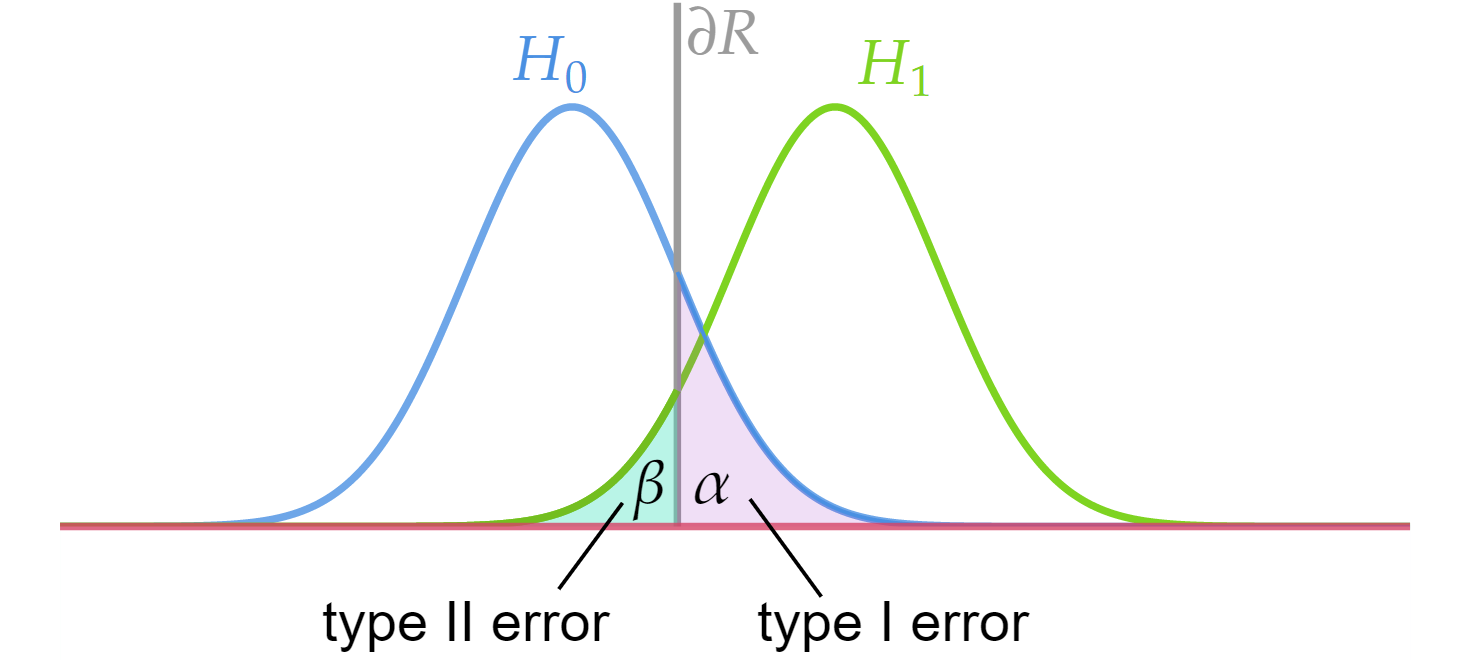
\includegraphics[width=0.55\linewidth]{sections/images/2022-09-05-16-16-51.png}
        \caption{Illustration of type I\&II error}
        \label{}
    \end{figure}
    

        
\begin{point}
        \textbf{Neyman-Pearson Principle}\index{Neyman-Pearson Principle}: First control $\alpha\leq\alpha_0$, then take $\min \beta$.
\end{point}


        How to determine $\alpha_0$? Depend on specific problem.\footnote{In most cases, take $\alpha_0=0.05$.}

        \item $p$-value: probability to get larger bias than observed $\vec{x}_0$ \uline{under $H_0$.}
        
        e.g. For reject region $R=\{\vec{X}|T(\vec{X})\geq C\},$ $p$-value:
        \begin{equation}
            p_{H_0}(\vec{x})=\mathbb{P}[T(\vec{X})\geq t(\vec{x}_0)|H_0]
        \end{equation}


        Remark: We believe that sample should reflect the property of model parameter, and $ p $-value is that under $H_0$, the probability to get a \textbf{worse} result than $\vec{x}$.
        
        Rule: Reject $H_0$ if $p(\vec{x}_0)\leq\alpha_0$.

        Note: $ p $-value is \textbf{different from} $ \alpha $ or type I error. $ p $-value is generated before we make decision while $ \alpha  $ arises after we decide how to make decisions. (But they do target the same result.)

        \item Power Function\index{Power Function}: (when $H_0$ is given), probability to reject $H_0$ by sampling.
        \begin{equation}
            \pi(\theta)=\begin{cases}
                \mathbb{P}(\text{type I error}),& \theta\in\Theta_0\\
                1-\mathbb{P}(\text{type II error}),& \theta\in\Theta_1
            \end{cases}
            =
            \begin{cases}
                \alpha(\theta),&\theta\in\Theta_0\\
                1-\beta(\theta),&\theta\in\Theta_1
            \end{cases}
        \end{equation}

        Express as test function:
        \begin{equation}
            \pi(\theta)=\mathbb{E}[\varphi(\vec{X})|\theta]
        \end{equation}

        A nice test: $\pi(\theta)$ small under $H_0$, large under $H_1$ (and grows very fast at the boundary of $ H_0 $ and $ H_1 $).
        \end{itemize}

        \begin{point}
            \textbf{General Steps of Hypothesis Testing:}
        \end{point}
        
        

        \begin{enumerate}[topsep=0pt]
            \item Propose $H_0\,\&\, H_1$.
            \item Determine $R$ (usually in the form of a statistic, e.g. $R=\{\vec{X}:T(\vec{X})\geq c\}$).
            \item Select a proper $\alpha$ (to determine $c$).
            \item Sampling, get sample (as well as $t(\vec{x})$), then 
            \begin{itemize}[topsep=-1pt,itemsep=-2pt]
                \item compare with $R$ and determine whether to reject/accept $H_0$, or
                \item calculate $ p $-value and determine whether to reject/accept$ H_0 $
            \end{itemize}
            
                
            

        \end{enumerate}

% \subsubsection{Hypotheses Testing for Common Distributions}
%     \begin{itemize}
%         \item Single normal distribution: $\vec{X}=(X_1,X_2,\ldots,X_n)$ i.i.d. from $N(\mu,\sigma^2)$
        
%         Testing $\mu$:


%     \end{itemize}

\subsubsection{Hypothesis Testing of Common Distributions}\label{SubSectionHypothesisTestingOfCommonDistributions}
    For some common distribution populations, determine rejection region $R$ under certain $H_0$ with confidence coefficient $\alpha$.

    Definition of necessary statistics see section {\autoref{SubSectionConfidenceIntervalForDistributions}}.

    \begin{enumerate}
        \item Single normal population:\index{t-test@$ t $-test}

        \begin{table}[H]
            \centering
            \renewcommand\arraystretch{1.2}
            \begin{tabularx}{\linewidth}{|c|c|c|Y|c|}
                \hline
                Condition&$H_0$&$H_1$&Testing Statistic $T$&Rejection Region $R$\\
                \hline
                \multirow{3}{*}{$\sigma^2$ known, test $\mu$}&$\mu=\mu_0$&$\mu\neq\mu_0$&\multirow{3}{*}{$T=\dfrac{\sqrt{n}(\bar{X}-\mu_0)}{\sigma}\sim N(0,1)$}&$|T|>N_\frac{\alpha}{2}$\\
                &$\mu\leq\mu_0$&$\mu>\mu_0$&&$T>N_\alpha$\\
                &$\mu\geq\mu_0$&$\mu<\mu_0$&&$T<-N_\alpha$\\
                \hline
                \multirow{3}{*}{$\sigma^2$ unknown, test $\mu$}&$\mu=\mu_0$&$\mu\neq\mu_0$&\multirow{3}{*}{$T=\dfrac{\sqrt{n}(\bar{X}-\mu_0)}{S}\sim t_{n-1}$}&$|T|>t_{n-1,\frac{\alpha}{2}}$\\
                &$\mu\leq\mu_0$&$\mu>\mu_0$&&$T>t_{n-1,\alpha}$\\
                &$\mu\geq\mu_0$&$\mu<\mu_0$&&$T<-t_{n-1,\alpha}$\\
                \hline
                \multirow{3}{*}{$\mu$ known, test $\sigma^2$}&$\sigma^2=\sigma_0^2$&$\sigma^2\neq\sigma_0^2$&\multirow{3}{*}{$T=\dfrac{nS_\mu^2}{\sigma_0^2}\sim \chi_n^2$}&$T<\chi^2_{n,1-\frac{\alpha}{2}}\cup T>\chi^2_{n,\frac{\alpha}{2}}$\\
                &$\sigma^2\leq\sigma_0^2$&$\sigma^2>\sigma_0^2$&&$T>\chi^2_{n,\alpha}$\\
                &$\sigma^2\geq\sigma_0^2$&$\sigma^2<\sigma_0^2$&&$T<\chi^2_{n,1-\alpha}$\\
                \hline
                \multirow{3}{*}{$\mu$ unknown, test $\sigma^2$}&$\sigma^2=\sigma_0^2$&$\sigma^2\neq\sigma_0^2$&\multirow{3}{*}{$T=\dfrac{(n-1)S^2}{\sigma_0^2}\sim \chi_{n-1}^2$}&$T<\chi^2_{n-1,1-\frac{\alpha}{2}}\cup T>\chi^2_{n-1,\frac{\alpha}{2}}$\\
                &$\sigma^2\leq\sigma_0^2$&$\sigma^2>\sigma_0^2$&&$T>\chi^2_{n-1,\alpha}$\\
                &$\sigma^2\geq\sigma_0^2$&$\sigma^2<\sigma_0^2$&&$T<\chi^2_{n-1,1-\alpha}$\\
                \hline
            \end{tabularx}
        \end{table}


    \item Double normal population:
    
    \begin{table}[htbp]
        \centering
        \renewcommand\arraystretch{1.2}
        \begin{tabularx}{\linewidth}{|c|c|c|Y|c|}
            \hline
            Condition&$H_0$&$H_1$&Testing Statistic $T$&Rejection Region $R$\\
            \hline
            \multirow{3}{*}{\makecell{$\sigma_1^2,\sigma_2^2$ known,\\test $\mu_1-\mu_2$}}&$\mu_1-\mu_2=\mu_0$&$\mu_1-\mu_2\neq\mu_0$&\multirow{3}{*}{$T=\dfrac{\bar{X}-\bar{Y}-\mu_0}{\sqrt{\dfrac{\sigma_1^2}{m}+\dfrac{\sigma_2^2}{n}}}\sim N(0,1)$}&$|T|>N_\frac{\alpha}{2}$\\
                &$\mu_1-\mu_2\leq\mu_0$&$\mu_1-\mu_2>\mu_0$&&$T>N_\alpha$\\
                &$\mu_1-\mu_2\geq\mu_0$&$\mu_1-\mu_2<\mu_0$&&$T<-N_\alpha$\\
                \hline
                \multirow{3}{*}{\makecell{$\sigma_1^2,\sigma_2^2$ unknown,\\test $\mu_1-\mu_2$}}&$\mu_1-\mu_2=\mu_0$&$\mu_1-\mu_2\neq\mu_0$&\multirow{3}{*}{\makecell{$T=\dfrac{\bar{X}-\bar{Y}-\mu_0}{S_\omega}\sqrt{\dfrac{mn}{m+n}}$\\$\sim t_{m+n-2}$}}&$|T|>t_{m+n-2,\frac{\alpha}{2}}$\\
                &$\mu_1-\mu_2\leq\mu_0$&$\mu_1-\mu_2>\mu_0$&&$T>t_{m+n-2,\alpha}$\\
                &$\mu_1-\mu_2\geq\mu_0$&$\mu_1-\mu_2<\mu_0$&&$T<-t_{m+n-2,\alpha}$\\
                \hline
                \multirow{3}{*}{\makecell{$\mu_1,\mu_2$ known,\\test $\dfrac{\sigma^2_1}{\sigma_2^2}$}}&$\sigma_1^2=\sigma_2^2$&$\sigma_1^2\neq\sigma_2^2$&\multirow{3}{*}{$T=\dfrac{S_{\mu_2}^2}{S_{\mu_1}^2}\sim F_{n,m}$}&\makecell{$T<F_{n,m,1-\frac{\alpha}{2}}$\\$\cup \,T>F_{n,m,\frac{\alpha}{2}}$}\\
                &$\sigma_1^2\geq\sigma_2^2$&$\sigma_1^2<\sigma_2^2$&&$T>F_{n,m,\alpha}$\\
                &$\sigma_1^2\leq\sigma_2^2$&$\sigma_1^2>\sigma_2^2$&&$T<F_{n,m,1-\alpha}$\\
                \hline
                \multirow{3}{*}{\makecell{$\mu_1,\mu_2$ unknown,\\test $\dfrac{\sigma^2_1}{\sigma_2^2}$}}&$\sigma_1^2=\sigma_2^2$&$\sigma_1^2\neq\sigma_2^2$&\multirow{3}{*}{$T=\dfrac{S_{2}^2}{S_{2}^2}\sim F_{n-1,m-1}$}&\makecell{$T<F_{n-1,m-1,1-\frac{\alpha}{2}}$\\$\cup\, T>F_{n-1,m-1,\frac{\alpha}{2}}$}\\
                &$\sigma_1^2\geq\sigma_2^2$&$\sigma_1^2<\sigma_2^2$&&$T>F_{n-1,m-1,\alpha}$\\
                &$\sigma_1^2\leq\sigma_2^2$&$\sigma_1^2>\sigma_2^2$&&$T<F_{n-1,m-1,1-\alpha}$\\
                \hline
        \end{tabularx}
    \end{table}

    \item None normal population:
    
    \begin{table}[htbp]
        \centering
        \renewcommand\arraystretch{1.7}
        \begin{tabularx}{\linewidth}{|c|c|c|Y|c|}
            \hline
            Condition&$H_0$&$H_1$&Testing Statistic $T$&Rejection Region $R$\\
            \hline
            \makecell{$\vec{X}$ from $B(1,p)$, test $p$}&$p=p_0$&$p\neq p_0$&$T=\dfrac{\sqrt{n}(\bar{X}-p_0)}{\sqrt{p_0(1-p_0)}}\xrightarrow[]{\mathscr{L}}N(0,1)$&$|T|>N_\frac{\alpha}{2}$\\
            \hline
            \makecell{$\vec{X}$ from $P(\lambda)$, test $\lambda$}&$\lambda=\lambda_0$&$\lambda\neq \lambda_0$&$T=\dfrac{\sqrt{n}(\bar{X}-\lambda_0)}{\sqrt{\lambda_0}}\xrightarrow[]{\mathscr{L}}N(0,1)$&$|T|>N_\frac{\alpha}{2}$\\
            \hline
        \end{tabularx}
    \end{table}
    \item More than two normal population: Analysis of Variance.
\end{enumerate}

\subsubsection{Likelihood Ratio Test}\label{SubSectionLRT}
    \index{LRT (Likelihood Ratio Test)}
    Idea: To test $H_0:\theta\in\Theta_0\longleftrightarrow H_1:\theta\in\Theta_1$ known $\vec{x}$, examine the likelihood function $L(\theta;\vec{x})$ and \textbf{compare} $L_{\theta\in\Theta_0}$ and $L_{\theta\in\Theta}$ to see the likelihood that $H_0$ is true.

    Def. \textbf{Likelihood Ratio} (LR):
    \begin{equation}
    \Lambda (\vec{x})=\dfrac{{\displaystyle\sup_{\theta\in\Theta_0}L(\theta;\vec{x})}}{{\displaystyle\sup_{\theta\in\Theta}L(\theta;\vec{x})}}
    \end{equation}

    Reject $H_0$ if $\Lambda(\vec{x})<\Lambda_0$. Or equivalently: Reject $H_0$ if $-2\ln\Lambda(\vec{x})>C(=-2\ln\Lambda_0)$.

    where $\Lambda_0$ (or equivalently $C=-2\ln\Lambda_0$) satisfies:
    \begin{equation}\mathbb{E}_{\Theta_0}[\varphi(\vec{X})]\leq\alpha,\quad\forall\theta\in\Theta_0\end{equation}

    LR and sufficient statistic: $\Lambda(\vec{x})$ can be expressed as $\Lambda(\vec{x})=\Lambda^*(T(\vec{x}))$, where $T(\vec{X})$ is sufficient statistic.


\begin{point}
    LRT for one-sample $ t $-test: For $ X_1,X_2,\ldots,X_n $ i.i.d. $ \sim N(\mu,\sigma ^2) $, test

\[
    H_0: \mu=\mu_0\longleftrightarrow H_1:\mu\neq\mu_0\quad\text{when }\sigma ^2\text{ unknown}
\]

    Can prove:
    \[
        \Lambda^{2/n}=\dfrac{\sum\limits_{i=1}^n(x_i-\bar{x})^2}{\sum\limits_{i=1}^n(x_i-\mu_0)^2} 
    \]
    
    Denote $ T=\dfrac{\sqrt{n}(\bar{x}-\mu_0)}{S}$, then LRT is
    \[
        \Lambda = \left( 1+\dfrac{T^2}{n-1} \right)^{-n/2}
    \]
    
    The Multivariate case see {\autoref{SubSectionMultivariateHypothesisTesting}}, where $ T^2 $ itself is the Hotelling's $ T^2 $ statistic.
    
    

\end{point}



\begin{point}
    Limiting Distribution of LRT: Wilks' Thm.\index{Wilk's Thm.}
\end{point}

    

    
    If $\dim\Theta=k>\dim\mathrm{span}\{\Theta_0\}=s$\footnote{Here 'dimension' refers to 'degree of freedom'.}, then under $H_0:\theta\in\Theta_0$:
    \begin{equation}
        \Lambda_{\theta\in\Theta_0}(\vec{x})=-2\ln \lambda(\vec{x})\xrightarrow[]{\mathscr{L}}\chi_{k-s}^2
    \end{equation}

\subsubsection{Uniformly Most Powerful Test}\label{SUbSectionUMP}
    \index{UMPT (Uniformly Most Powerful Test)}Idea: Neyman-Pearson Principle: control $\alpha$, find $\min\beta$. i.e. control $\alpha$, find $\max\pi(\theta)$

    Def. \textbf{Uniformly Most Powerful Test} (UMP) $\varphi_{\mathrm{UMP}}$ with level of significance $\alpha$ satisfies
    \begin{equation}
        \pi_{\mathrm{UMP}}(\theta)\geq\pi(\theta),\,\forall\theta\in\Theta_1
    \end{equation}

    \textbf{Neyman-Pearson Lemma}\index{NP-Lemma (Neyman-Pearson Lemma)}: For $\vec{X}=(X_1,X_2,\ldots,X_n)$ i.i.d. from $f(\vec{x};\theta)$. 
    
    Test hypothesis $H_0:\theta=\theta_0\longleftrightarrow H_1:\theta=\theta_1$. Def. test function $\varphi$ as:
    \begin{equation}\label{UMPtestfunction}
        \varphi(\vec{x})=\begin{cases}
            1,&\dfrac{f(\vec{x};\theta_1)}{f(\vec{x};\theta_0)}>C\\
            r,&\dfrac{f(\vec{x};\theta_1)}{f(\vec{x};\theta_0)}=C\\
            0,&\dfrac{f(\vec{x};\theta_1)}{f(\vec{x};\theta_0)}<C
        \end{cases}
    \end{equation}

    Then there exists $C$ and $r$ such that
    \begin{itemize}
        \item $\mathbb{E}[\varphi(\vec{x})|\theta_0]=\mathbb{P}(\dfrac{f(\vec{x};\theta_1)}{f(\vec{x};\theta_0)}>C)+r\mathbb{P}(\dfrac{f(\vec{x};\theta_1)}{f(\vec{x};\theta_0)}=C)=\alpha$
        \item This $\varphi$ is UMP of level of significance $\alpha$
    \end{itemize}

    Actually kind of $1$-dimensional case of LRT.

    Note: UMT exist for\textbf{ simple }$H_0,H_1$, otherwise may not exist.

    UMP and sufficient statistics: Test function $\varphi(\vec{X})$ given by \autoref{UMPtestfunction} is function of sufficient statistics $T(\vec{X})$, i.e. $\varphi(\vec{X})=\varphi^*(T(\vec{X}))$.

    UMP and Exponential Family: For sample $\vec{X}=(X_1,X_2,\dots,X_n)$ from exponential family:
    \begin{equation}
    f(\vec{x};\theta)=C(\theta)h(\vec{x})\exp\{Q(\theta)T(\vec{x})\}    
    \end{equation}

    Test single hypothesis $H_0:\theta=\theta_0\longleftrightarrow H_1:\theta=\theta_1$, (where $ \theta_0<\theta_1 $ ).
    If 
    \begin{itemize}[topsep=0.5pt,itemsep=0pt]
        \item $\theta_0$ is inner point of $\Theta$
        \item $Q(\theta)$  monotone increase with $\theta$
    \end{itemize}

    Then UMP exists, in the form of:
    \begin{equation}\label{UMPtestfunctioninExponentialFamily}
            \varphi(\vec{x})=\begin{cases}
        1,&T(\vec{x})>C\\
        r,&T(\vec{x})=C\\
        0,&T(\vec{x})<C
    \end{cases} 
    \end{equation}
   
    

    where $C$ and $r$ satisfies $\mathbb{E}[\varphi(\vec{x})|\theta_0]=\alpha$.

    Note: or take $Q(\theta)$ mono decreased, then in \autoref{UMPtestfunctioninExponentialFamily}, take opposite inequality operators.
    
\begin{point}
    \textbf{General Steps of UMP}:
\end{point}

    
    \begin{enumerate}
        \item Find a point $\theta_0\in\Theta_0$ and a point $\theta_1\in\Theta_1$. (Note: \textbf{one} point)
        \item Construct test function in the form of {\autoref{UMPtestfunction}}, use $\mathbb{E}[\varphi(\vec{x})|\theta_0]=\alpha$ to determine $C$ and $r$.
        \item Get $R$ and $\varphi(\vec{x})$.
        \item If $\varphi$ does \textbf{not} depend on $\theta_1$, then $H_1$ can be generalized to $H_1:\theta\in\Theta_1$.
        \item If $\varphi$ satisfies $\mathbb{E}_{\theta\in\Theta_0}(\varphi)\leq\alpha$, then $H_0$ an be generalized to $H_0:\theta\in\Theta_0$.
    \end{enumerate}

\subsubsection{Duality of Hypothesis Testing and Interval Estimation}

\begin{itemize}
    \item Thm.: $\forall\theta_0\in\Theta$ there exists hypothesis testing $H_0:\theta=\theta_0\longleftrightarrow H_1:\theta\neq\theta_0$ of level $\alpha$ with rejection region $R_{\theta_0}$. Then
    \begin{equation}
        C(\vec{X})=\{\theta:\vec{X}\in R^C_{\theta}\}
    \end{equation}

    is a $1-\alpha$ confidence region for $\theta$

    \item Thm.: $C(\vec{X})$ is a $1-\alpha$ confidence region for $\theta$. Then $\forall\theta_0\in C(\vec{X})$, the rejection region of hypothesis testing $H_0:\theta=\theta_0\longleftrightarrow H_1:\theta\neq\theta_0$ of level $\alpha$ satisfies
    \begin{equation}
    R^\complement_{\theta_0}=\{\vec{X}:\theta_0\in C(\vec{X})\}
    \end{equation}
\end{itemize}
    
    \begin{point}
        Idea:
    \end{point}
    
        
\begin{itemize}[itemsep=-3pt]
    \item[] \centering $H_0:\theta=\theta_0\longleftrightarrow H_1:\theta\neq\theta_0$
    \begin{equation}\updownarrow\end{equation}
    \item[] \centering $\mathbb{P}(R^\complement(\vec{X})|H_0)=\mathbb{P}(R^\complement(\vec{X})|\theta_0)=1-\alpha$
    \begin{equation}\updownarrow\end{equation}
    \item[] Confidence Interval: $\theta_0\in R^\complement(\vec{X})$
\end{itemize}

    Similar for Confidence Limit and One-Sided Testing.

\subsubsection{Introduction to Non-Parametric Hypothesis Testing}\label{SubSectionIntroToNonParametricHypothesisTesting}

    Motivation: Usually distribution form unknown, cannot use parametric hypothesis testing.

    Useful Method:
    \begin{itemize}
        \item Sign Test: Used for paired comparison $\vec{X}=(X_1,X_2,\ldots,X_n)$, $\vec{Y}=(Y_1,Y_2,\ldots,Y_n)$.
        
        Take $Z_i=Y_i-X_i$ i.i.d., denote $E(Z)=\mu$. Test $H_0:\mu=0\longleftrightarrow H_1:\mu\neq 0$.

        Denote $n_+=\#(\text{positive } Z_i)$ and $n_-=\#(\text{negative }Z_i)$, $n_0=n_++n_-$. Then $n_+\sim B(n_0,\theta)$, test $H_0:\theta=\dfrac{1}{2}\longleftrightarrow H_1:\theta\neq\dfrac{1}{2}$
        
        Then use Binomial Testing or large sample CLT Normal Testing.

        Remark:
        \begin{itemize}
            \item Also can test $H_0:\theta\leq\dfrac{1}{2}\longleftrightarrow H_1:\theta>\dfrac{1}{2}$
            \item Drawback: ignores magnitudes.
        \end{itemize}
        
        \item \index{WSRT (Wilcoxon Signed Rank Sum Test)}Wilcoxon Signed Rank Sum Test: Improvement of Sign Test. Base on order statistics.
        
        Order Statistics of $Z_i$: $Z_{(1)}<Z_{(2)}<\ldots<Z_{(n)}$, where each $Z_{(j)}$ corresponds to some $Z_i$, denote as $Z_i=Z_{(R_i)}$, then $R_i$ is the rank of $Z_i$.\footnote{If some $X_i,X_j,\ldots$ equal, then take same rank $R=\mathrm{mean}\{R_i,R_j,\ldots\}$.}
        
        Def. $\vec{R}=(R_1,R_2,\ldots,R_n)$ is \textbf{Rank Statistics} of $(Z_1,Z_2,\ldots,Z_n)$

        Def. \textbf{Sum of Wilcoxon Signed Rank}: 
        \begin{equation}
        W^+=\sum_{i=1}^{n_0}R_i\mathbb{I}_{Z_i>0} 
        \end{equation}

        Distribution of $W^+$ is complex. $E$ and $var$ of $W^+$ under $H_0$:
        \begin{equation}
            \mathbb{E}(W^+)=\frac{n_0(n_0+1)}{4}\qquad var(W^+)=\frac{n_0(n_0+1)(2n_0+1)}{24}    
        \end{equation}

        Usually consider large sample CLT, construct normal approximation:
        \begin{equation}
            T=\frac{W^+-\mathbb{E}(W^+)}{\sqrt{var(W^+)}}\xrightarrow[]{\mathscr{L}}N(0,1)
        \end{equation}

        Rejection Region: $R=\{|T|>N_\frac{\alpha}{2}\}$

        \item Wilcoxon Two-Sample Rank Sum Test: Used for two independent sample comparison.\index{Wilcoxon Two-Sample Rank Sum Test}
        
        Assume $\vec{X}=(X_1,\ldots,X_m)$ i.i.d. $\sim f(x)$; $\vec{Y}=(Y_1,\ldots,Y_n)$ i.i.d. $\sim f(x-\theta)$, test $H_0:\theta=0\longleftrightarrow H_1:\theta\neq 0$.

        Rank $X_i$ and $Y_i$ as:
        \begin{equation}
            Z_1\leq Z_2\leq\ldots\leq Z_{m+n}
        \end{equation}

        in which denote rank of $Y_i$ as $R_i$, and def. \textbf{Wilcoxon two-sample rank sum}:
        \begin{equation}W=\sum_{i=1}^n R_i\end{equation}

        $\mathbb{E}$ and $var$ of $W$ under $H_0$:
\begin{equation}\mathbb{E}(W)=\frac{n(m+n+1)}{2}\qquad var(W)=\frac{mn(n+m+1)}{12}\end{equation}

        Use large sample approximation, construct CLT:
        \begin{equation}
            T=\frac{W-\mathbb{E}(W)}{\sqrt{var(W)}}\xrightarrow[]{\mathscr{L}}N(0,1)
        \end{equation}







        \item Goodness-of-Fit Test: For $\vec{X}=(X_1,X_2,\ldots,X_n)$ i.i.d. from some certain population $X$. Test $H_0:X\sim F(x)$.\index{Goodness-of-Fit Test}
        
        where $F$ is theoretical distribution, can be either parametric or non-parametric.

        Idea: Define some \textit{quantity} $D=D(X_1,\ldots,X_n;F)$ to measure the difference between $F$ and sample. And def. \textit{Goodness-of-fit} when observed value of $D$ (say $d_0$) is given:
        \begin{equation}p(d_0)=\mathbb{P}(D\geq d_0|H_0)\end{equation}

        \textbf{Goodness-of-Fit Test}: Reject $H_0$ if $p(d_0)<\alpha$.


            Pearson $\chi^2$ Test: Usually used for discrete case. 
            
            Test $H_0:\mathbb{P}(X_i=a_i)=p_i,\, i=1,2,\ldots,r$. Denote $\#(X_j=a_i)=\nu_i$, take $D$ as:
            \begin{equation}\label{Pearson_chi_test_differenceKn}
                K_n=K_n(X_1,\ldots,X_n;F)=\sum_{i=1}^r\frac{(\nu_i-np_i)^2}{np_i}
            \end{equation}

            Pearson Thm.: For $K_n$ defined as \autoref{Pearson_chi_test_differenceKn}, then under $H_0$:
            \begin{equation}
                K_n\xrightarrow[]{\mathscr{L}}\chi^2_{r-1-s}
            \end{equation} 

            Here $s$ is number of unknown parameter, $r-1-s$ is the degree of freedom.

            Note:
            \begin{itemize}
                \item $a_i$ must \textbf{not} depend on sample.
                \item For continuous case, construct division:
                \begin{equation}\mathbb{R}\rightarrow(-\infty,a_1,a_2,\ldots,a_{r-1},\infty=a_r) \end{equation}

                and test $H_0:\mathbb{P}(X\in I_j)=p_j$

                Criterion: Pick proper interval so that $np_i$ and $\nu_i$ both $\geq 5$.
            \end{itemize}
 


        \item Contingency Table Independence \& Homogeneity Test
        \index{Contingency Table}
 
\begin{itemize}
    \item Independence Test:\index{Pearson's $ \chi^2 $ Test}
    
    Test a two-parameter sample and to see whether these two parameters(features) are independent. Denote $Z=(X,Y)$ are some 'level' of sample, $n_{ij}$ is number of sample with level $(i,j)$

    Contingency Table:
    \begin{table}[H]
        \centering
        \begin{tabular}{|c|ccccc|c|}
            \hline
            \diagbox{X}{Y}&1&$\ldots$&$j$&$\ldots$&$s$&$\sum$\\
            \hline
            1&$n_{11}$&$\ldots$&$n_{1j}$&$\ldots$&$n_{1s}$&$n_{1\cdot}$\\
            $\vdots$&$\vdots$&$\ddots$&$\vdots$&$\ddots$&$\vdots$&$\vdots$\\
            $i$&$n_{i1}$&$\ldots$&$n_{ij}$&$\ldots$&$n_{is}$&$n_{i\cdot}$\\
            $\vdots$&$\vdots$&$\ddots$&$\vdots$&$\ddots$&$\vdots$&$\vdots$\\
            $r$&$n_{r1}$&$\ldots$&$n_{rj}$&$\ldots$&$n_{rs}$&$n_{r\cdot}$\\
            \hline
            $\sum$&$n_{\cdot 1}$&$\ldots$&$n_{\cdot j}$&$\ldots$&$n_{\cdot s}$&$n$\\
            \hline
        \end{tabular}
    \end{table}

        Test $H_0:X\,\&\, Y$ are independent. i.e. $H_0:P(X=i,Y=j)=P(X=i)P(Y=j)=p_{i\cdot}p_{\cdot j}$.

        Construct $\chi^2$ test statistic:
        \begin{equation}
            K_n=\sum_{i=1}^r\sum_{j=1}^s\frac{[n_{ij}-n(\frac{n_{i\cdot}}{n})(\frac{n_{\cdot j}}{n})]^2}{n(\frac{n_{i\cdot}}{n})(\frac{n_{\cdot j}}{n})}=n\left(\sum_{i=1}^r\sum_{j=1}^s\frac{n_{ij}^2}{n_{i\cdot}n_{\cdot j}}-1\right)
        \end{equation}

        Then under $H_0$, $K_n\xrightarrow[]{\mathscr{L}}\chi^2_{rs-1-(r+s-2)}=\chi^2_{(r-1)(s-1)}$

        Reject $H_0$ if $p(k_0)=P(K_n\geq k_0)<\alpha$


        \item Homogeneity Test:
        
        Test $R$ groups of sample with category rank, to see whether these groups has similar rank distribution.

        \begin{table}[H]
            \centering
            \begin{tabular}{|c|ccccc|c|}
                \hline
                \diagbox{Group}{Category}&Category 1&$\ldots$&Category $j$&$\ldots$&Category $C$&$\sum$\\
                \hline
                Group 1&$n_{11}$&$\ldots$&$n_{1j}$&$\ldots$&$n_{1C}$&$n_{1\cdot}$\\
                $\vdots$&$\vdots$&$\ddots$&$\vdots$&$\ddots$&$\vdots$&$\vdots$\\
                Group $i$&$n_{i1}$&$\ldots$&$n_{ij}$&$\ldots$&$n_{iC}$&$n_{i\cdot}$\\
                $\vdots$&$\vdots$&$\ddots$&$\vdots$&$\ddots$&$\vdots$&$\vdots$\\
                Group $R$&$n_{R1}$&$\ldots$&$n_{Rj}$&$\ldots$&$n_{RC}$&$n_{R\cdot}$\\
                \hline
                $\sum$&$n_{\cdot 1}$&$\ldots$&$n_{\cdot j}$&$\ldots$&$n_{\cdot C}$&$n$\\
                \hline
            \end{tabular}
        \end{table}


    Denote $P(\text{Category }j|\text{Group }i)=p_{ij}$. Test $H_0:p_{ij}=p_j,\,\forall 1\leq i\leq R$.

    Construct $\chi^2$ test statistic:
    \begin{equation}
        D=\sum_{i=1}^R\sum_{j=1}^C\frac{[n_{ij}-n(\frac{n_{i\cdot}}{n})(\frac{n_{\cdot j}}{n})]^2}{n(\frac{n_{i\cdot}}{n})(\frac{n_{\cdot j}}{n})}=n\left(\sum_{i=1}^R\sum_{j=1}^C\frac{n_{ij}^2}{n_{i\cdot}n_{\cdot j}}-1\right)
    \end{equation}

    Then under $H_0$, $D\xrightarrow[]{\mathscr{L}}\chi^2_{R(C-1)-(C-1)}=\chi^2_{(R-1)(C-1)}$
    \end{itemize}

    \item \hypertarget{testofnormality}{Test of Normality}: normality is a good \& useful assumption.
    
    For $\vec{Y}=(Y_1,Y_2,\ldots,Y_n)$,

    Test $H_0:\text{exists }\mu\,\&\, \sigma^2$ such that $Y_i$ i.i.d. $\sim N(\mu,\sigma^2)$.

    \begin{itemize}
        \item Kolmogorov-Smirnov Test\index{K-S Test (Kolmogorov-Smirnov Test)}: Assume $\vec{X}$ form population CDF $F(x)$, test $H_0:F(x)=F_0(x)$(where can take $F_0=\Phi$ or some other known CDF).
        
        use $F_n(x)$ (as defined in \autoref{empiricaldisreibutionfunction}) as approx. to $F(x)$, test
        \begin{equation}
            D_n=\sum_{-\infty< x<+\infty}|F_n(x)-F_0(x)|
        \end{equation}

        Reject $H_0$ if $D_n>c$

        or use goodness-of-fit: denote observed value of $D_n$ as $d_n$. Reject $H_0$ if
        \begin{equation}
            p(d_n)=\mathbb{P}(D_n>d_n|H_0)<\alpha
        \end{equation}

        \item Shapiro-Wilk Test:\index{S-W Test (Shapiro-Wilk Test)}
        
        Test $H_0:\text{exists }\mu\,\&\, \sigma^2$ such that $X_i$ i.i.d. $\sim N(\mu,\sigma^2)$.

        Denote $Y_{(i)}=\dfrac{X_{(i)}-\mu}{\sigma}$, $m_i=\mathbb{E}(Y_{(i)})$

        Under $H_0$, $(X_{(i)},m_i)$ falls close to straight line. Test Statistic: Correlation
        \begin{equation}
            R^2=\dfrac{\left(\sum_{i=1}^n(X_{(i)}-\bar{X})(m_i-\bar{m})\right)^2}{\sum_{i=1}^n(X_{i}-\bar{X})^2\sum_{i=1}^n(m_i-\bar{m})^2}=corr(X_{(i)},m_i)
        \end{equation}

        Reject $H_0$ if $R^2<c$

        Shapiro-Wilk correction:
        \begin{equation}
            W=\dfrac{\left(\sum_{i=1}^{[n/2]}a_i(X_{(n+1-i)}-X_{(i)})\right)^2}{\sum_{i=1}^n(X_{(i)}-\bar{X})^2}
        \end{equation}
    \end{itemize}
\end{itemize}

\begin{point}
    Summary: Useful Non-Parameter Hypothesis Testing.
\end{point}
\\
\\

\begin{equation*}
    \text{\makecell{Non-Parameter\\Hypothesis Testing}}
    \smash[htbp]{
    \begin{cases}
        \text{One Population Sample}
            \smash[t]{
                \begin{cases}
                    \chi^2\text{ Test}\\
                    \text{Binomial Test}\\
                    \text{One-Sample K-S Test}\\
                    \text{Wilcoxon Sign Test}\\
                    \text{Runs Test}
                \end{cases}
            }\\
            \\
            \\
            \\
            \\
        \text{Two Population Sample}
            \smash[t]{
                \begin{cases}
                    \text{Independent Sample}
                    \smash[t]{
                        \begin{cases}
                            \text{Mann-Whitney Test}\\
                            \text{K-S Test}\\
                            \text{Wald-Wolfowitz Test}\\
                            \text{Moses Test of Extreme Reactions}
                        \end{cases}
                    }\\
                    \\
                    \text{Relative Sample}
                    \smash[b]{
                        \begin{cases}
                            \text{Sign Test}\\
                            \text{McNemar Test}\\
                            \text{Wilcoxon Rank Sum Test}\\
                            \text{Marginal Homogeneity Test}
                        \end{cases}
                    }
                \end{cases}
            }\\
            \\
            \\
            \\
        \text{Multi-Population Sample}
            \smash[b]{
                \begin{cases}
                    \text{Independent Sample}
                    \smash[t]{
                        \begin{cases}
                            \text{Median Test}\\
                            \text{K-W One-Way ANOVA Test}\\
                            \text{Jonckheere-Terpstra Test}
                        \end{cases}
                    }\\
                    \\
                    \text{Relative Sample}
                    \smash[b]{
                        \begin{cases}
                            \text{Friedman Rank Sum Test}\\
                            \text{Kendall's Coefficient of Concordance Test}\\
                            \text{Cochran Q Test}
                        \end{cases}
                    }
                \end{cases}
            }
    \end{cases}  
    }
\end{equation*}
